\documentclass[a4paper,12pt]{article}
\usepackage{path}
\usepackage[spanish]{babel}
\usepackage{graphicx}
\graphicspath{{../img/}}
\usepackage[section]{placeins}
\usepackage{hyperref}
\hypersetup{
    colorlinks = true,
    linkcolor = blue,
    urlcolor = cyan
}
\usepackage[T1]{fontenc}
\usepackage[utf8]{inputenc} 
\usepackage{graphicx}
\usepackage{xcolor}
\usepackage{float}
\usepackage{enumitem}
\usepackage{booktabs}
\usepackage{geometry}
\usepackage{titlesec}
\usepackage{fancyhdr}
\usepackage{parskip}
\usepackage{microtype}
\usepackage{pmboxdraw}

\geometry{margin=2.5cm}
\setlength{\parskip}{1em}
\setlength{\parindent}{0pt}

\definecolor{myblue}{HTML}{005F9E}
\definecolor{mygray}{HTML}{4D4D4D}
\definecolor{mycyan}{HTML}{008B8B}


\usepackage{lmodern}
\renewcommand{\familydefault}{\sfdefault}

\titleformat{\section}
  {\Large\bfseries\color{myblue}}
  {\thesection}{1em}{}

\titleformat{\subsection}
  {\large\bfseries\color{myblue}}
  {\thesubsection}{1em}{}

\titleformat{\subsubsection}
  {\normalsize\bfseries\color{mygray}}
  {\thesubsubsection}{1em}{}

\pagestyle{fancy}
\fancyhf{}
\fancyhead[L]{\textit{Afondamento nas Competencias Profesionais}}
\fancyhead[R]{\thepage}
\renewcommand{\headrulewidth}{0.4pt}
\renewcommand{\headrule}{\hbox to\headwidth{\color{myblue}\leaders\hrule height \headrulewidth\hfill}}

\title{
    \vspace{2cm}
    {\Huge\textbf{Afondamento nas Competencias Profesionais}}\\[1em]
    {\Large\textbf{Práctica 1.5}}\\[1em]
    {\Large CI/CD - Coolify y Ngrok}
    \vspace{1.5cm}
}

\author{\Large Daniel Calvar Cruz\\[0.5em]\normalsize 2º CS DAM}
\date{\vspace{1cm}\today}


\begin{document}

\maketitle

\clearpage

\hypertarget{anchor-indice}{}
\tableofcontents
\newpage

\section{Introducción}
\hyperlink{anchor-indice}{\textbf{Volver}}\\

\textbf{- ENUNCIADO -}

- ENUNCIADO -

\textbf{Requisitos previos:}

\begin{itemize}
  \item Creación de VM:
    \begin{itemize}
      \item SO recomendado: Ubuntu.
    \end{itemize}
\end{itemize}

\clearpage

\section{Coolify, Ngrok}
\hyperlink{anchor-indice}{\textbf{Volver}}\\

Instalación de Coolify y Ngrok:

\url{https://coolify.io/}

\url{https://ngrok.com/}

Tan solo hay que seguir las instrucciones en pantalla. Importante en Ngrok, crear cuenta y añadir Authtoken.

\begin{figure}[h!]
    \centering
    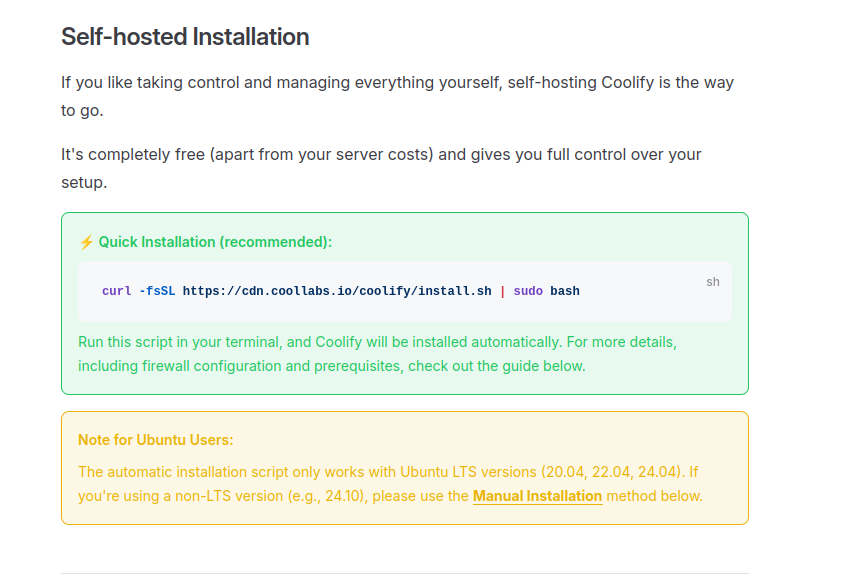
\includegraphics[width=1\textwidth]{01.png}
    \caption{Instalar Coolify}
\end{figure}
\FloatBarrier

\begin{figure}[h!]
    \centering
    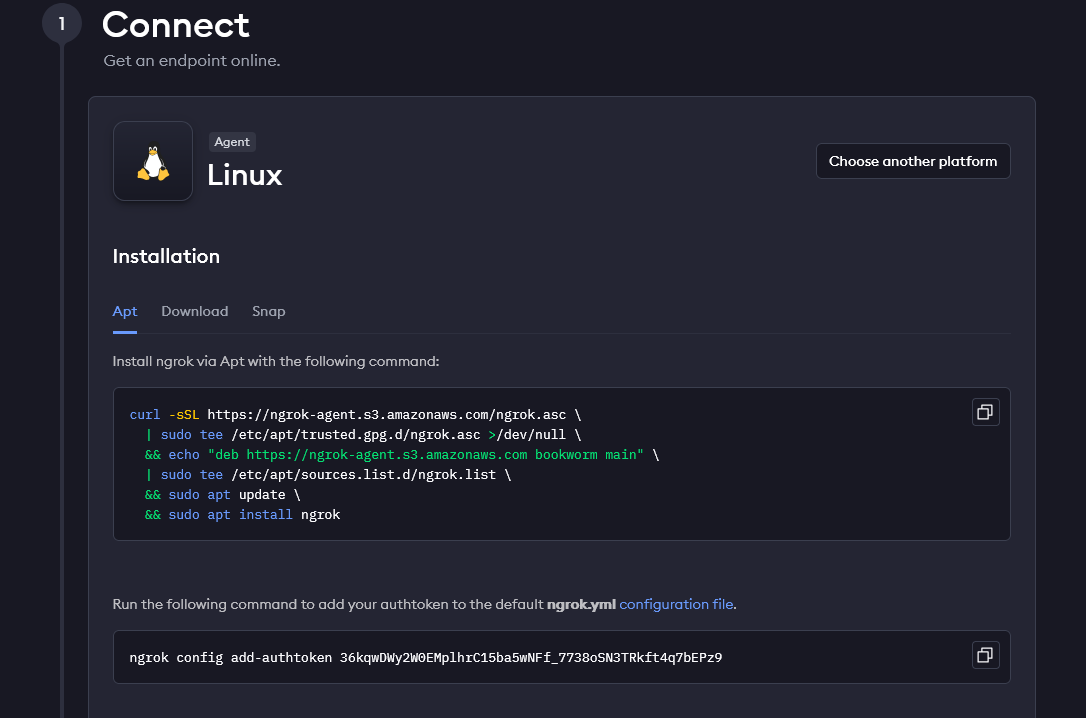
\includegraphics[width=1\textwidth]{03.png}
    \caption{Instalar Ngrok}
\end{figure}
\FloatBarrier

\clearpage

\section{Prueba con API test simple}
\hyperlink{anchor-indice}{\textbf{Volver}}\\

Ir al dashboard de Coolify (localhost:8000)

\begin{figure}[h!]
    \centering
    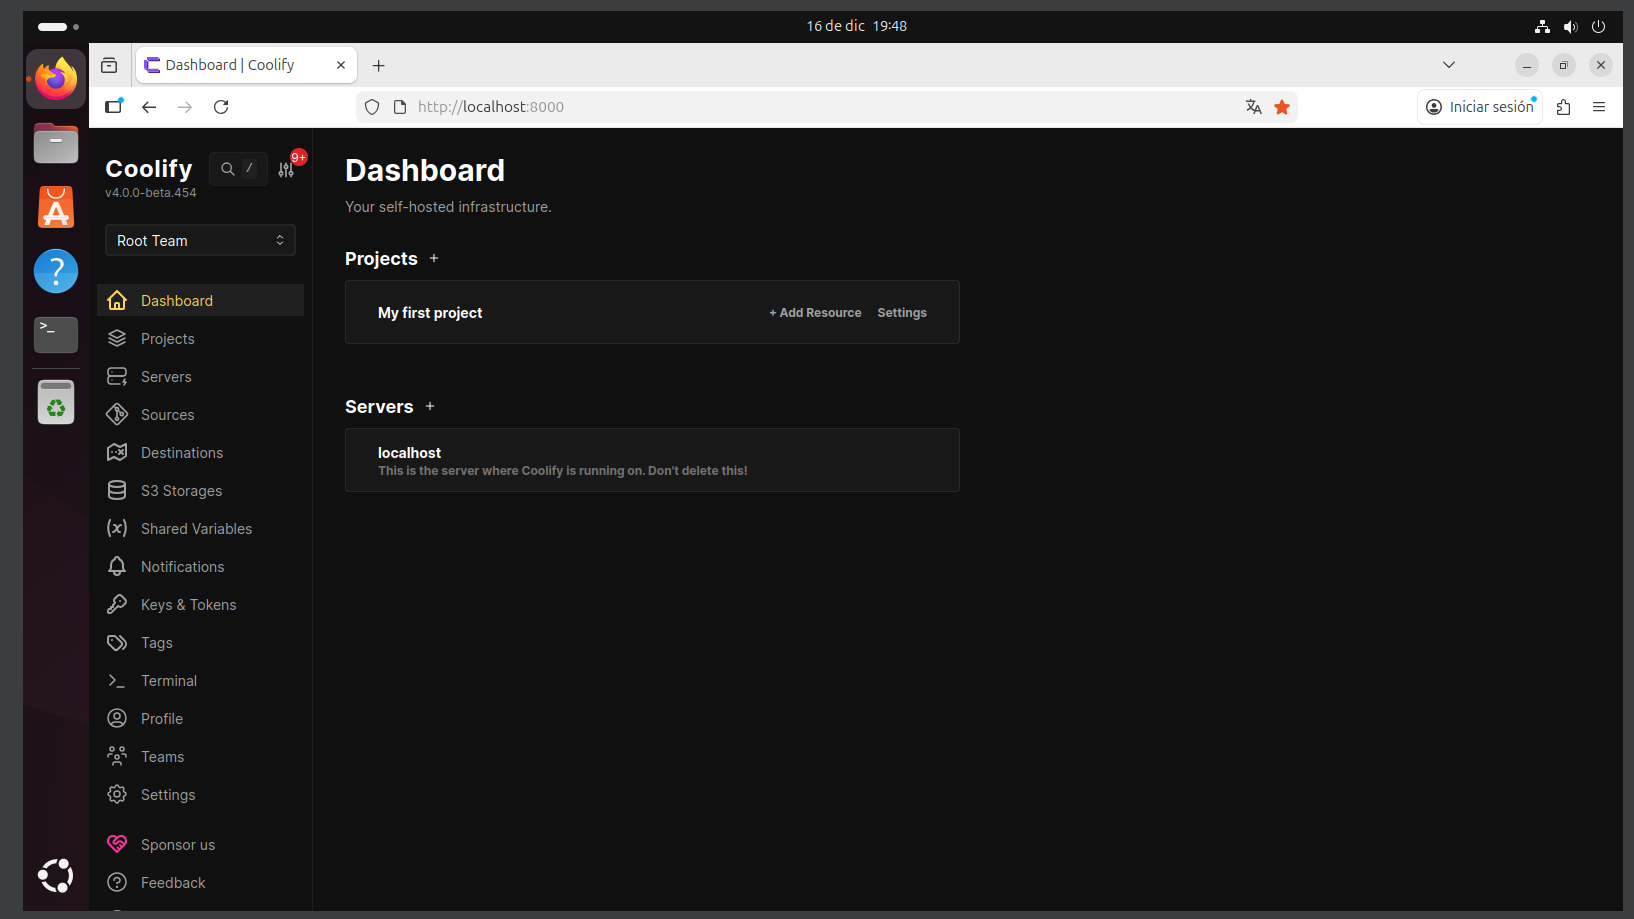
\includegraphics[width=1\textwidth]{04.png}
    \caption{Dashboard}
\end{figure}
\FloatBarrier

Crear nuevo proyecto, añadir recurso (repositorio público, \url{https://github.com/1001inchNails/apiTestCicd})

\begin{figure}[h!]
    \centering
    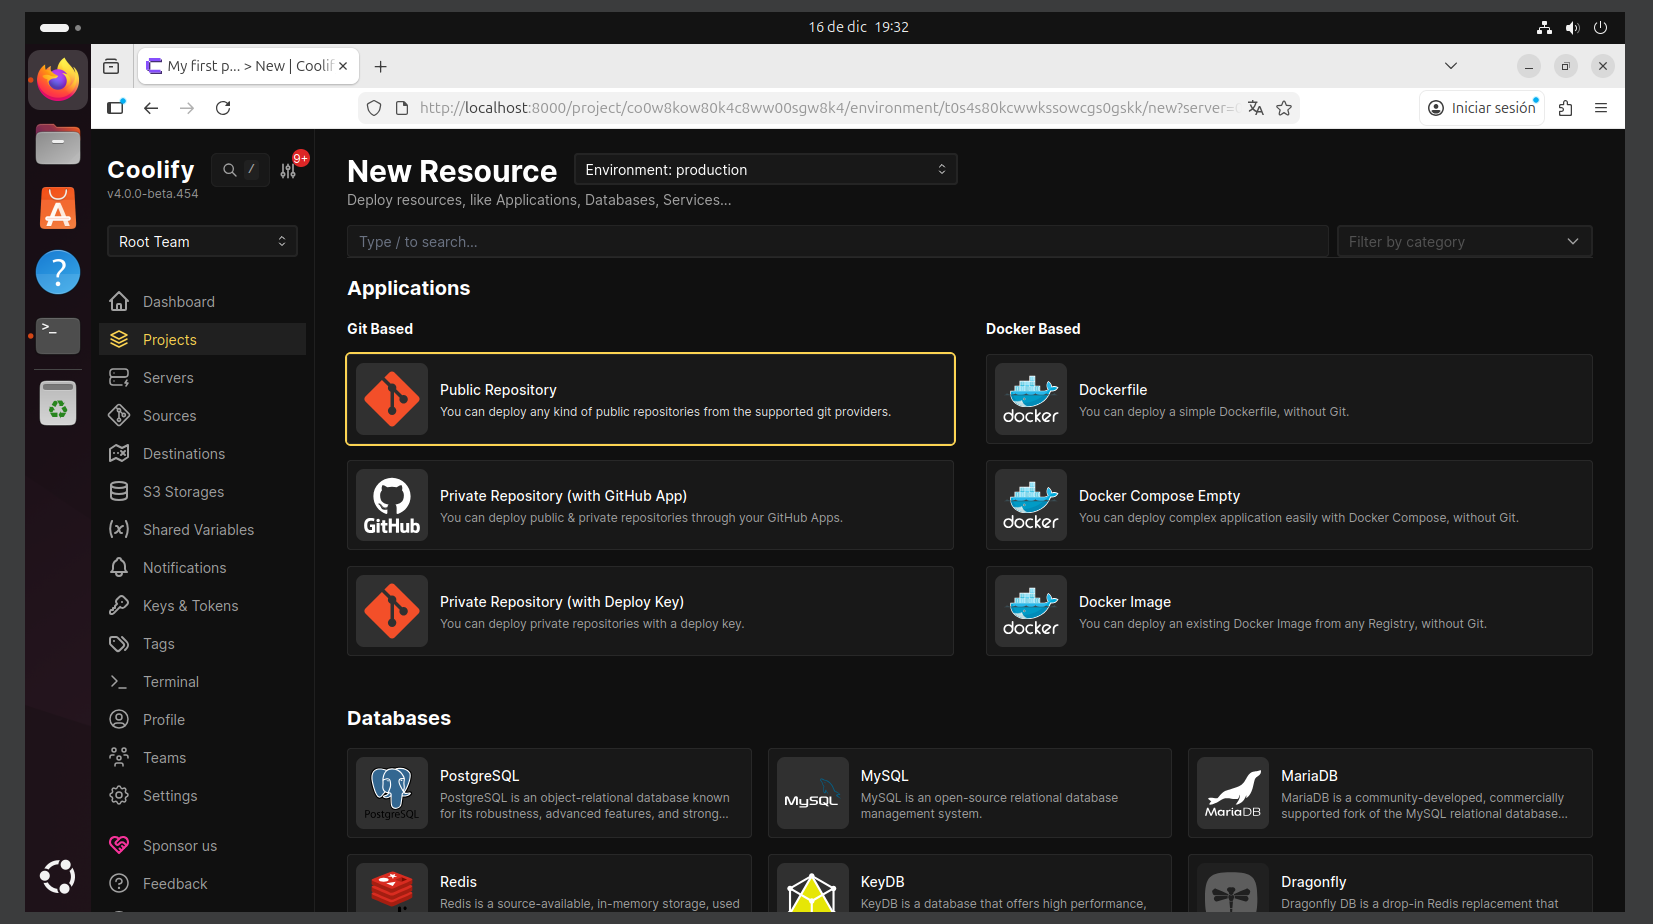
\includegraphics[width=1\textwidth]{05.png}
    \caption{Añadir recurso}
\end{figure}
\FloatBarrier

\begin{figure}[h!]
    \centering
    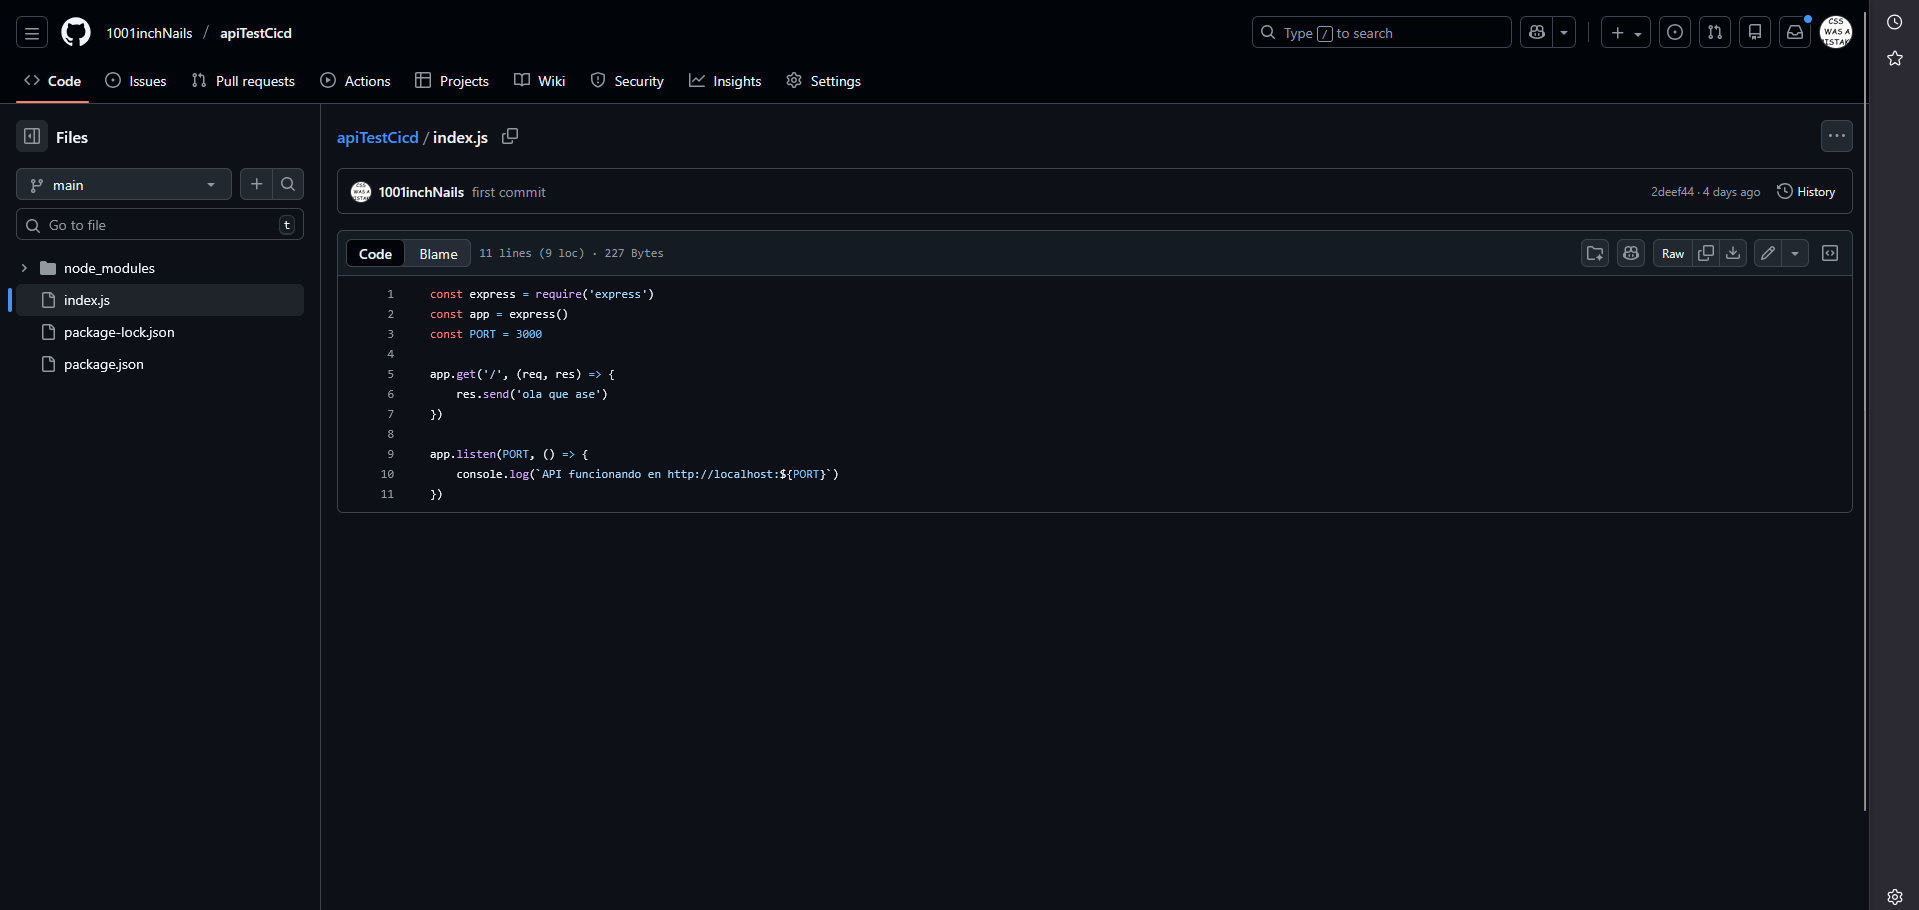
\includegraphics[width=1\textwidth]{07.png}
    \caption{Test API}
\end{figure}
\FloatBarrier

\begin{figure}[h!]
    \centering
    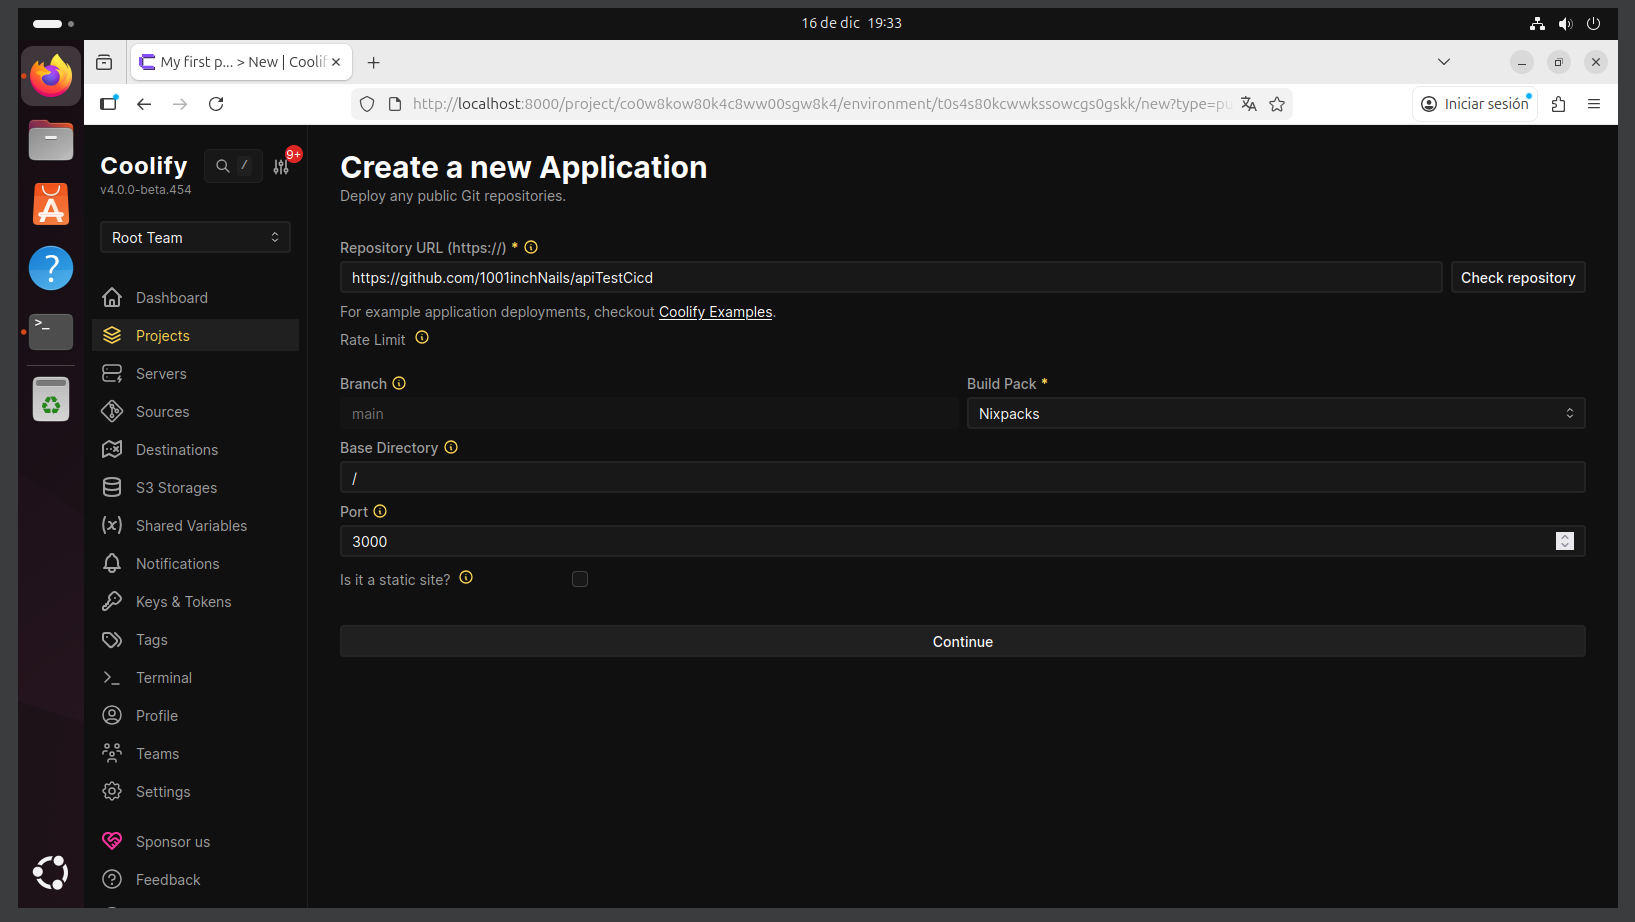
\includegraphics[width=1\textwidth]{06.png}
    \caption{Nixpacks, puerto 3000}
\end{figure}
\FloatBarrier

\begin{figure}[h!]
    \centering
    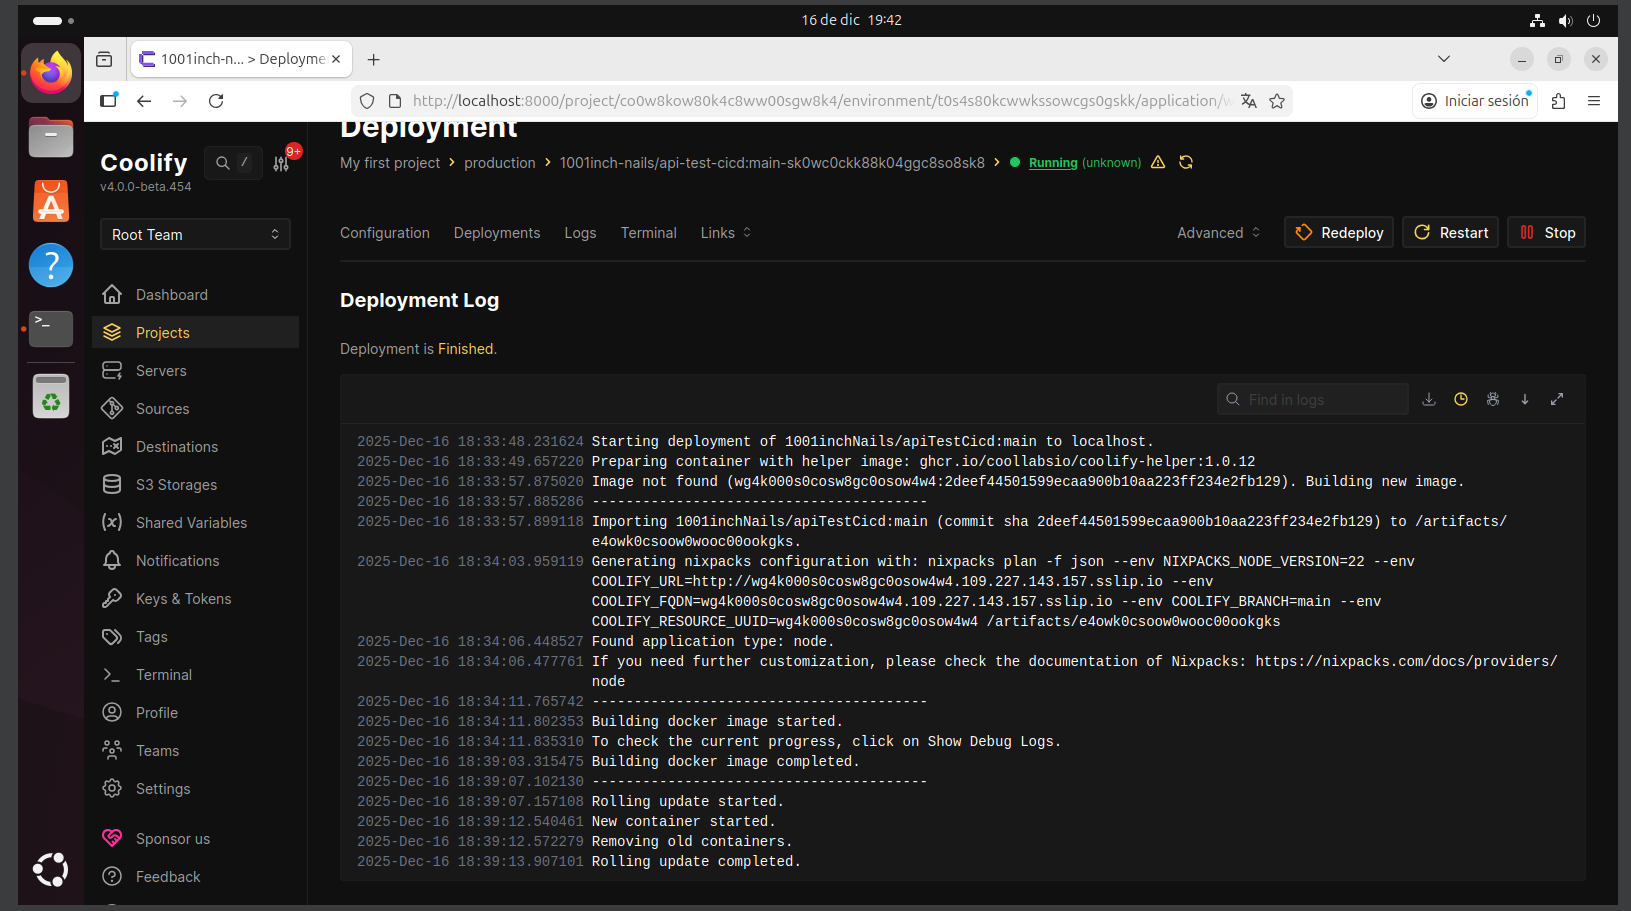
\includegraphics[width=1\textwidth]{08.png}
    \caption{Desplegar la API}
\end{figure}
\FloatBarrier

\begin{figure}[h!]
    \centering
    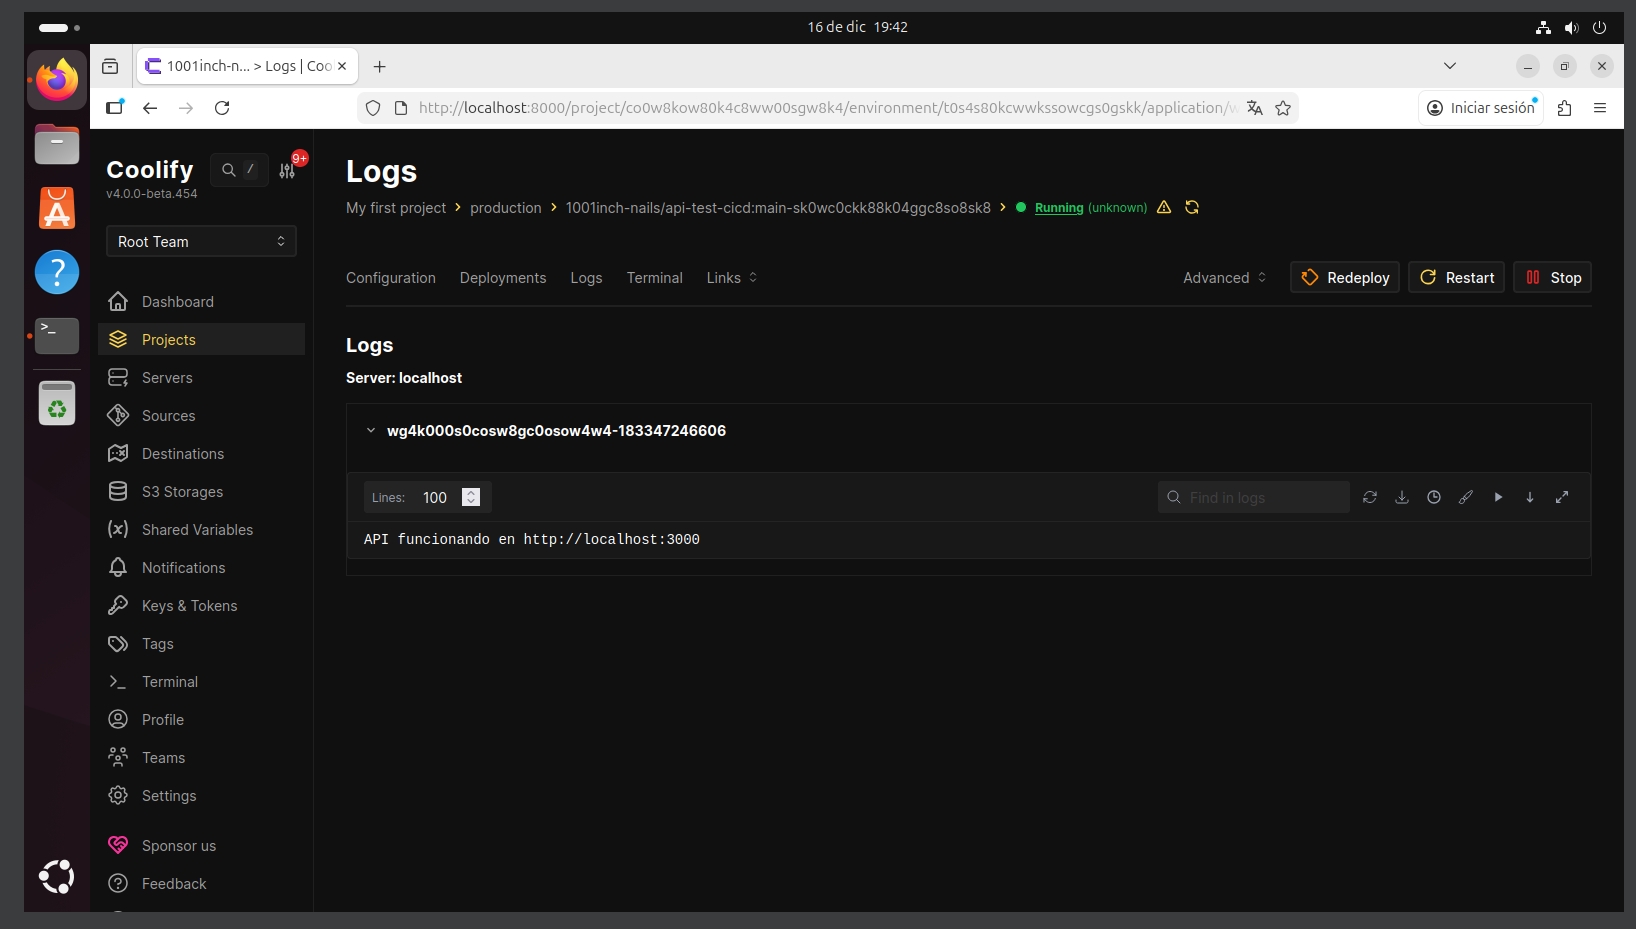
\includegraphics[width=1\textwidth]{09.png}
    \caption{Comprobar logs}
\end{figure}
\FloatBarrier

Buscamos la ID del contenedor con nuestra API:

\begin{figure}[h!]
    \centering
    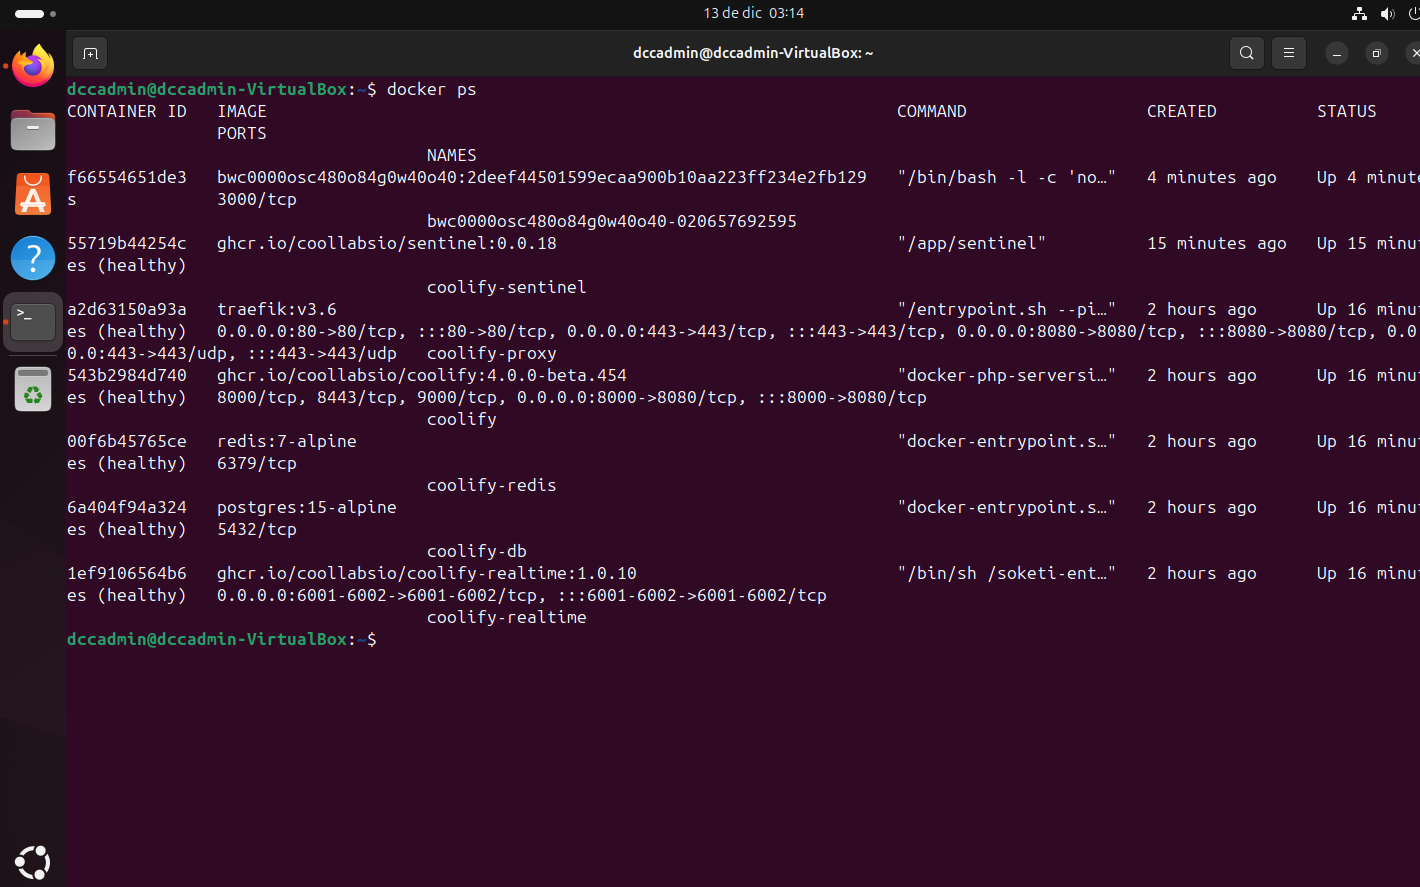
\includegraphics[width=1\textwidth]{10.png}
    \caption{En este caso, el primero}
\end{figure}
\FloatBarrier

Con esa ID, buscamos la IP del contenedor:

\begin{figure}[h!]
    \centering
    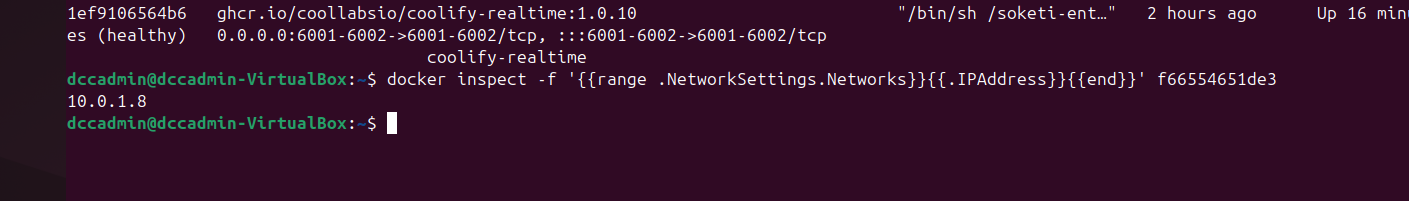
\includegraphics[width=1\textwidth]{11.png}
    \caption{IP del contenedor con nuestra API}
\end{figure}
\FloatBarrier

Comprobación en máquina local:

\begin{figure}[h!]
    \centering
    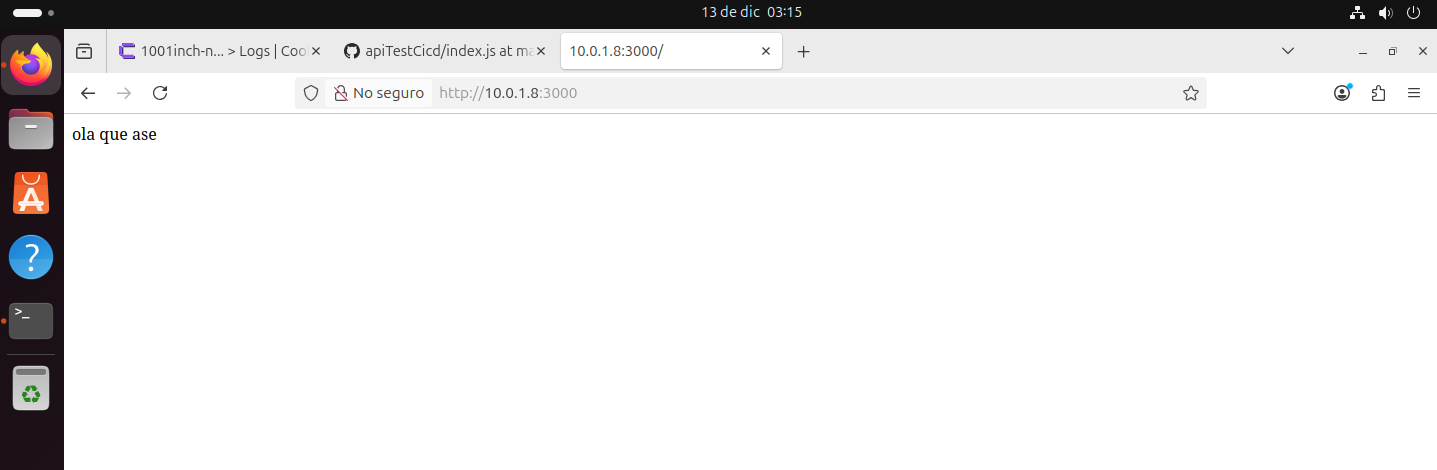
\includegraphics[width=1\textwidth]{12.png}
    \caption{Comprobación}
\end{figure}
\FloatBarrier

Exponemos con Ngrok:

\begin{figure}[h!]
    \centering
    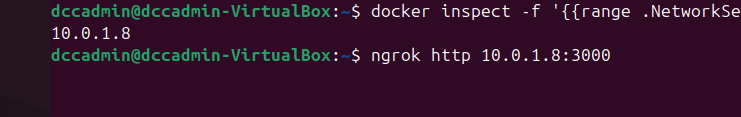
\includegraphics[width=1\textwidth]{13.png}
    \caption{Creación de "túnel" para exponer la API de local a exterior}
\end{figure}
\FloatBarrier

\begin{figure}[h!]
    \centering
    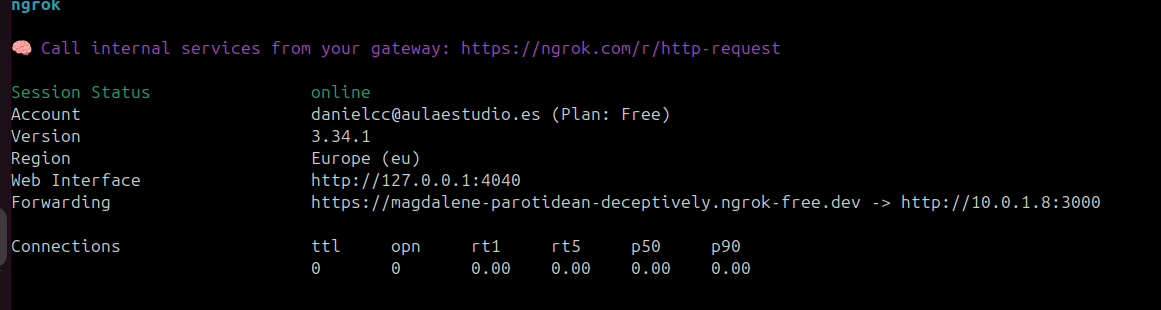
\includegraphics[width=1\textwidth]{14.png}
    \caption{No cerrar el terminal}
\end{figure}
\FloatBarrier

\begin{figure}[h!]
    \centering
    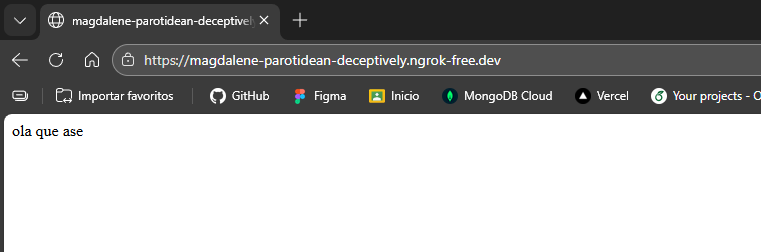
\includegraphics[width=1\textwidth]{16.png}
    \caption{Prueba en maquina host}
\end{figure}
\FloatBarrier

\clearpage

\section{Prueba con API/BBDD}
\hyperlink{anchor-indice}{\textbf{Volver}}\\

La práctica se desarrollará desde la máquina host, para ello exponemos el puerto 8000, usado por el dashboard de Coolify:

\begin{figure}[h!]
    \centering
    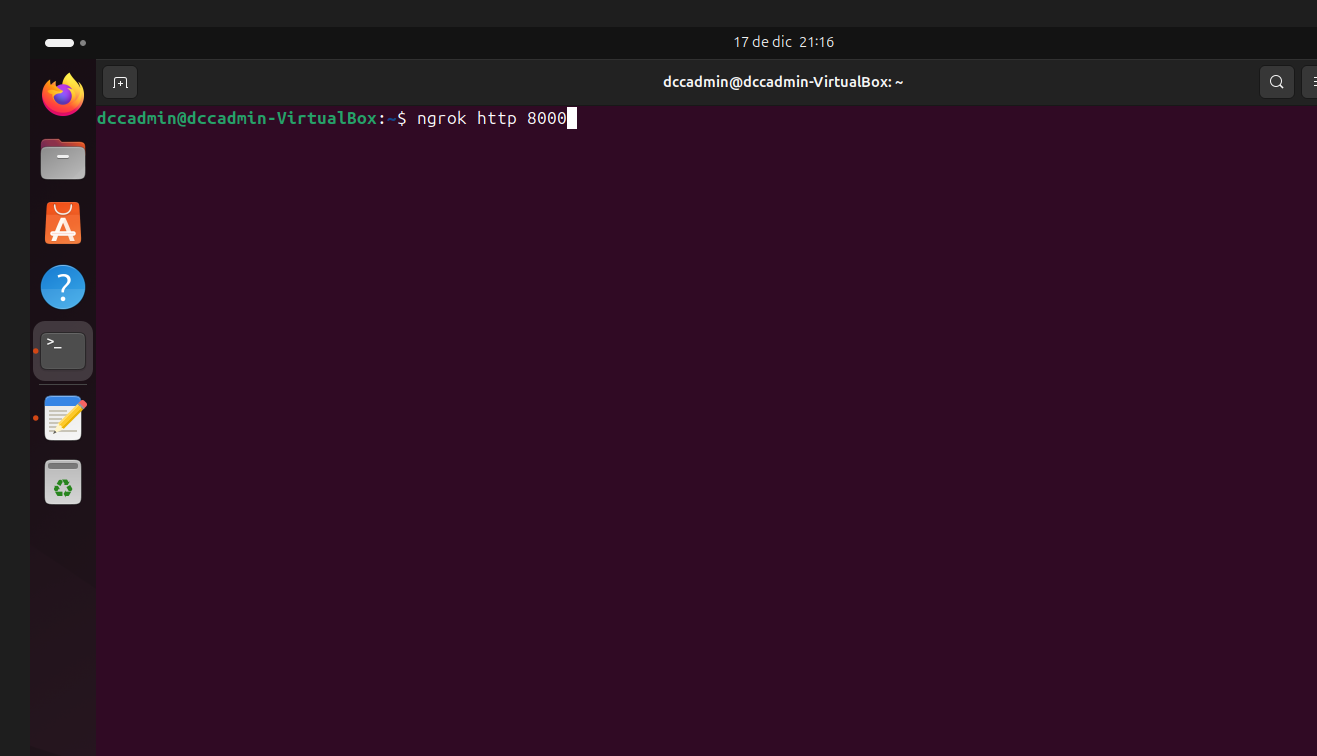
\includegraphics[width=1\textwidth]{17.png}
    \caption{Exponer puerto}
\end{figure}
\FloatBarrier

\begin{figure}[h!]
    \centering
    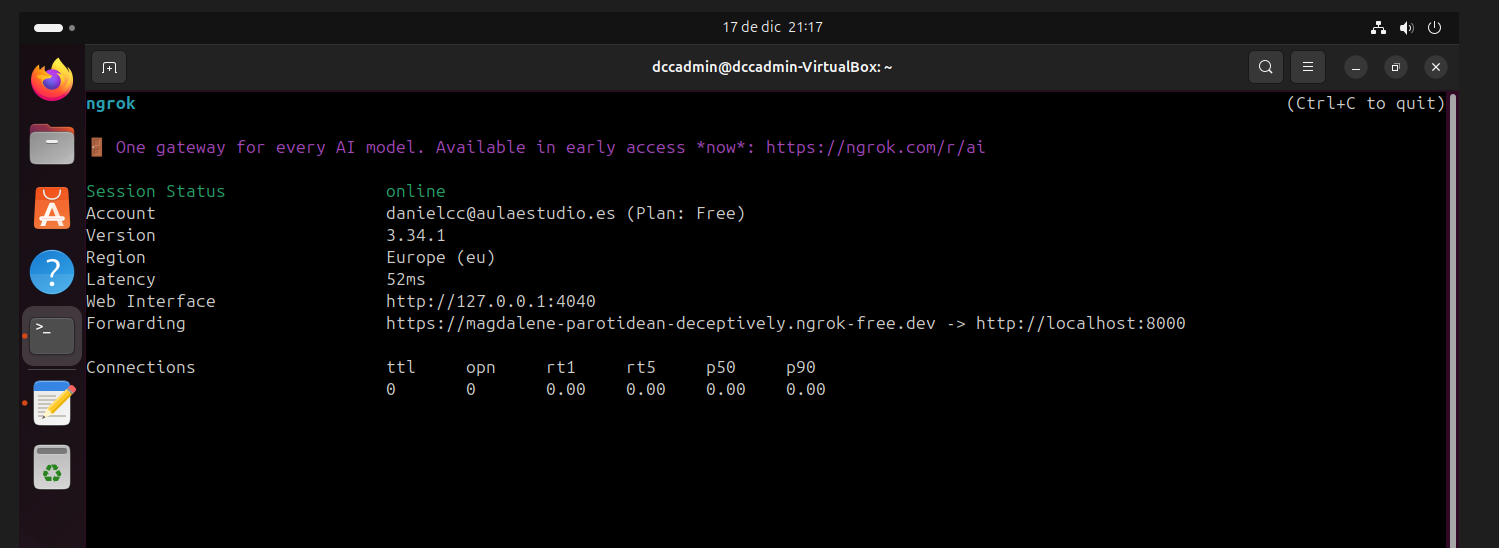
\includegraphics[width=1\textwidth]{18.png}
    \caption{Tunel}
\end{figure}
\FloatBarrier

\begin{figure}[h!]
    \centering
    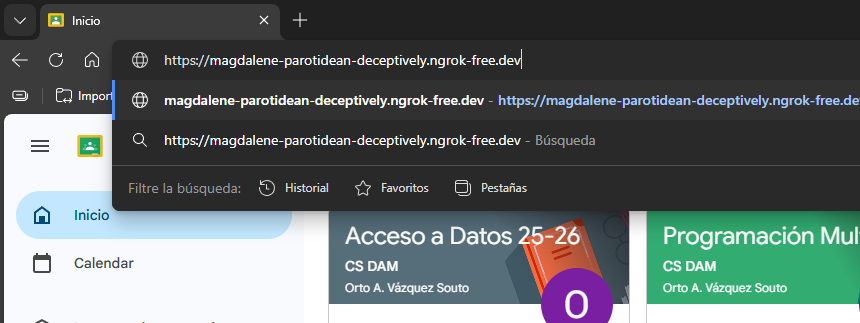
\includegraphics[width=1\textwidth]{19.png}
    \caption{En host}
\end{figure}
\FloatBarrier

\begin{figure}[h!]
    \centering
    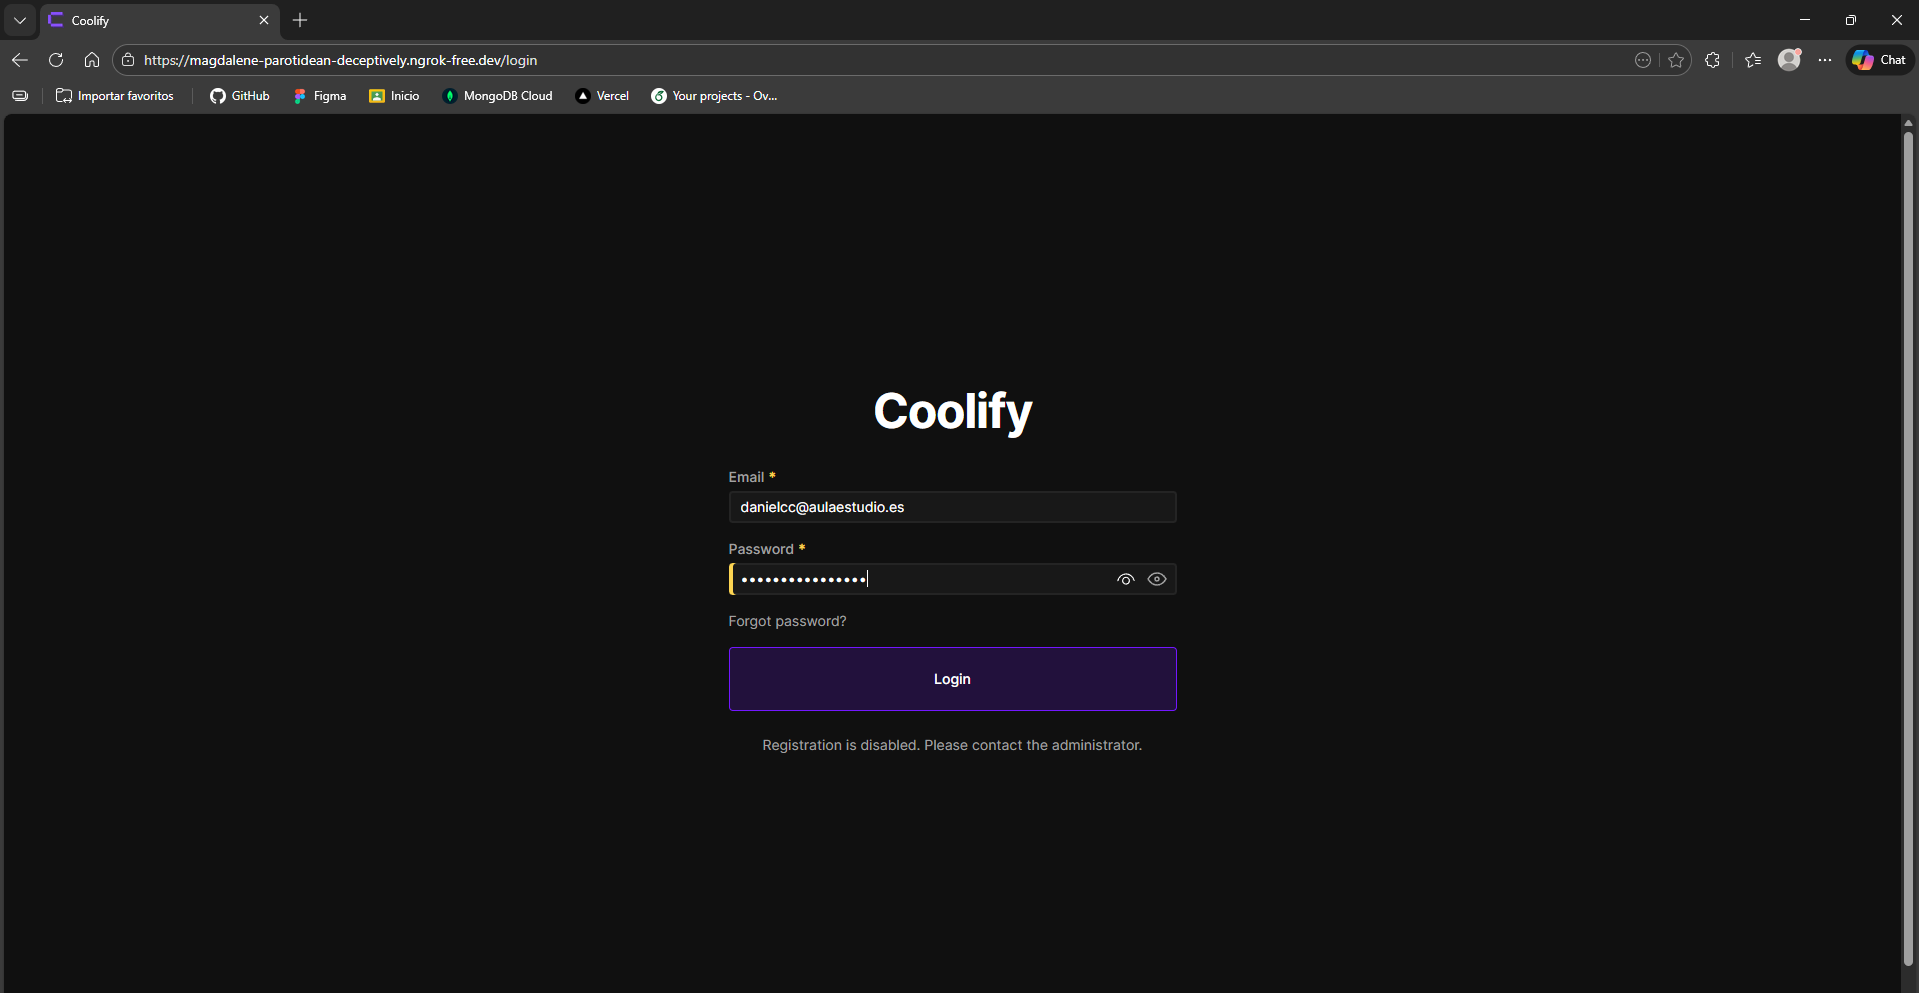
\includegraphics[width=1\textwidth]{20.png}
    \caption{Acceso a dashboard}
\end{figure}
\FloatBarrier

\begin{figure}[h!]
    \centering
    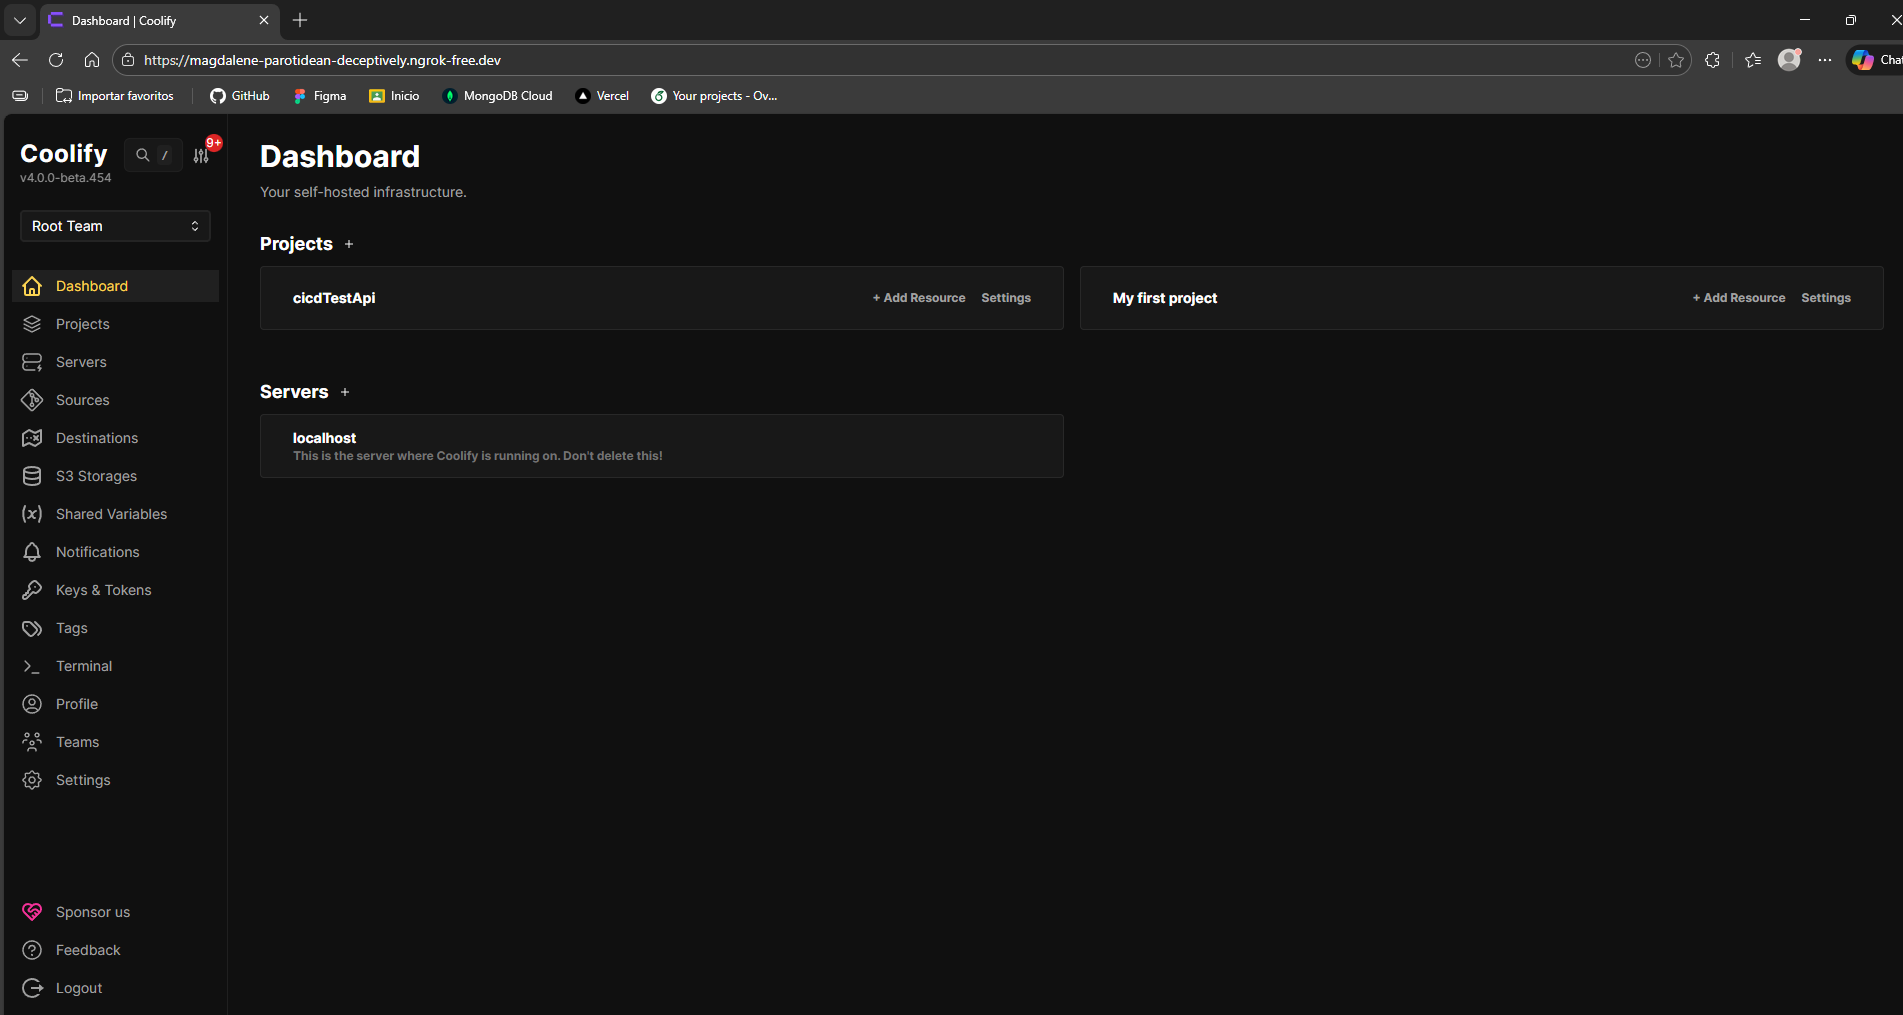
\includegraphics[width=1\textwidth]{21.png}
    \caption{Dashboard de Coolify de VM en máquina host}
\end{figure}
\FloatBarrier

Creamos un nuevo proyecto:

\begin{figure}[h!]
    \centering
    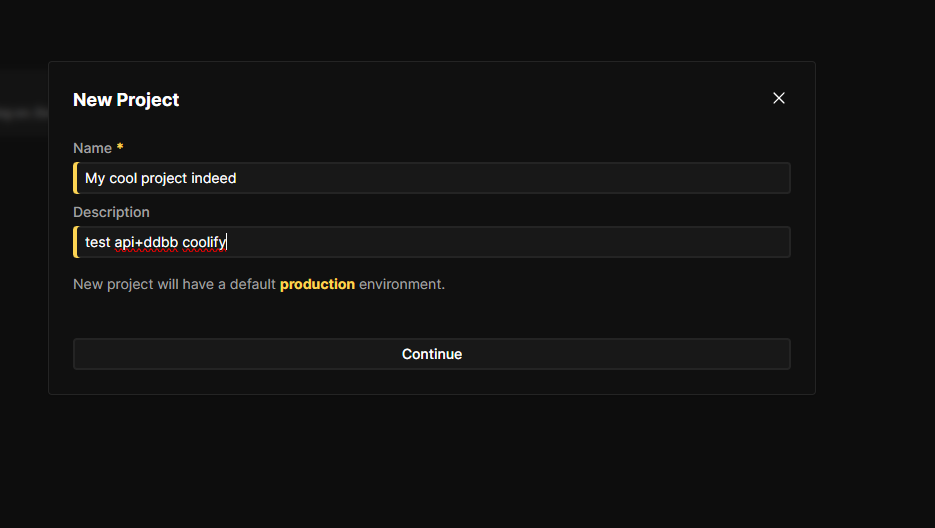
\includegraphics[width=1\textwidth]{22.png}
    \caption{Crear nuevo proyecto}
\end{figure}
\FloatBarrier

\begin{figure}[h!]
    \centering
    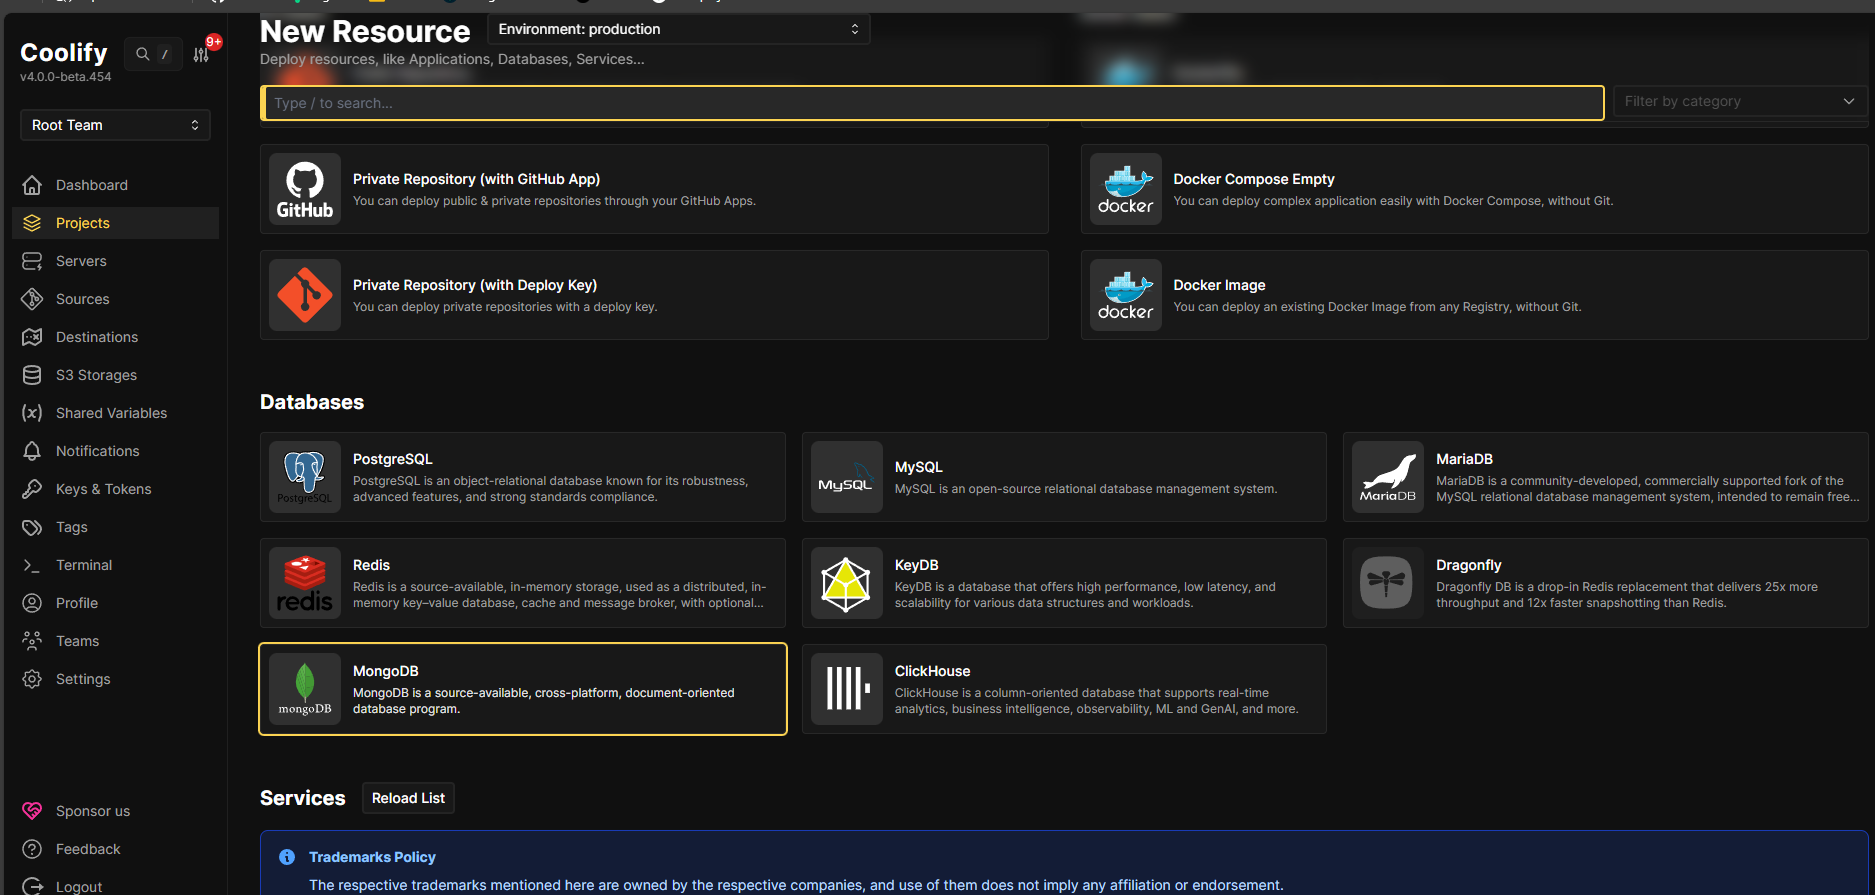
\includegraphics[width=1\textwidth]{23.png}
    \caption{Añadimos recurso: BBDD}
\end{figure}
\FloatBarrier

\begin{figure}[h!]
    \centering
    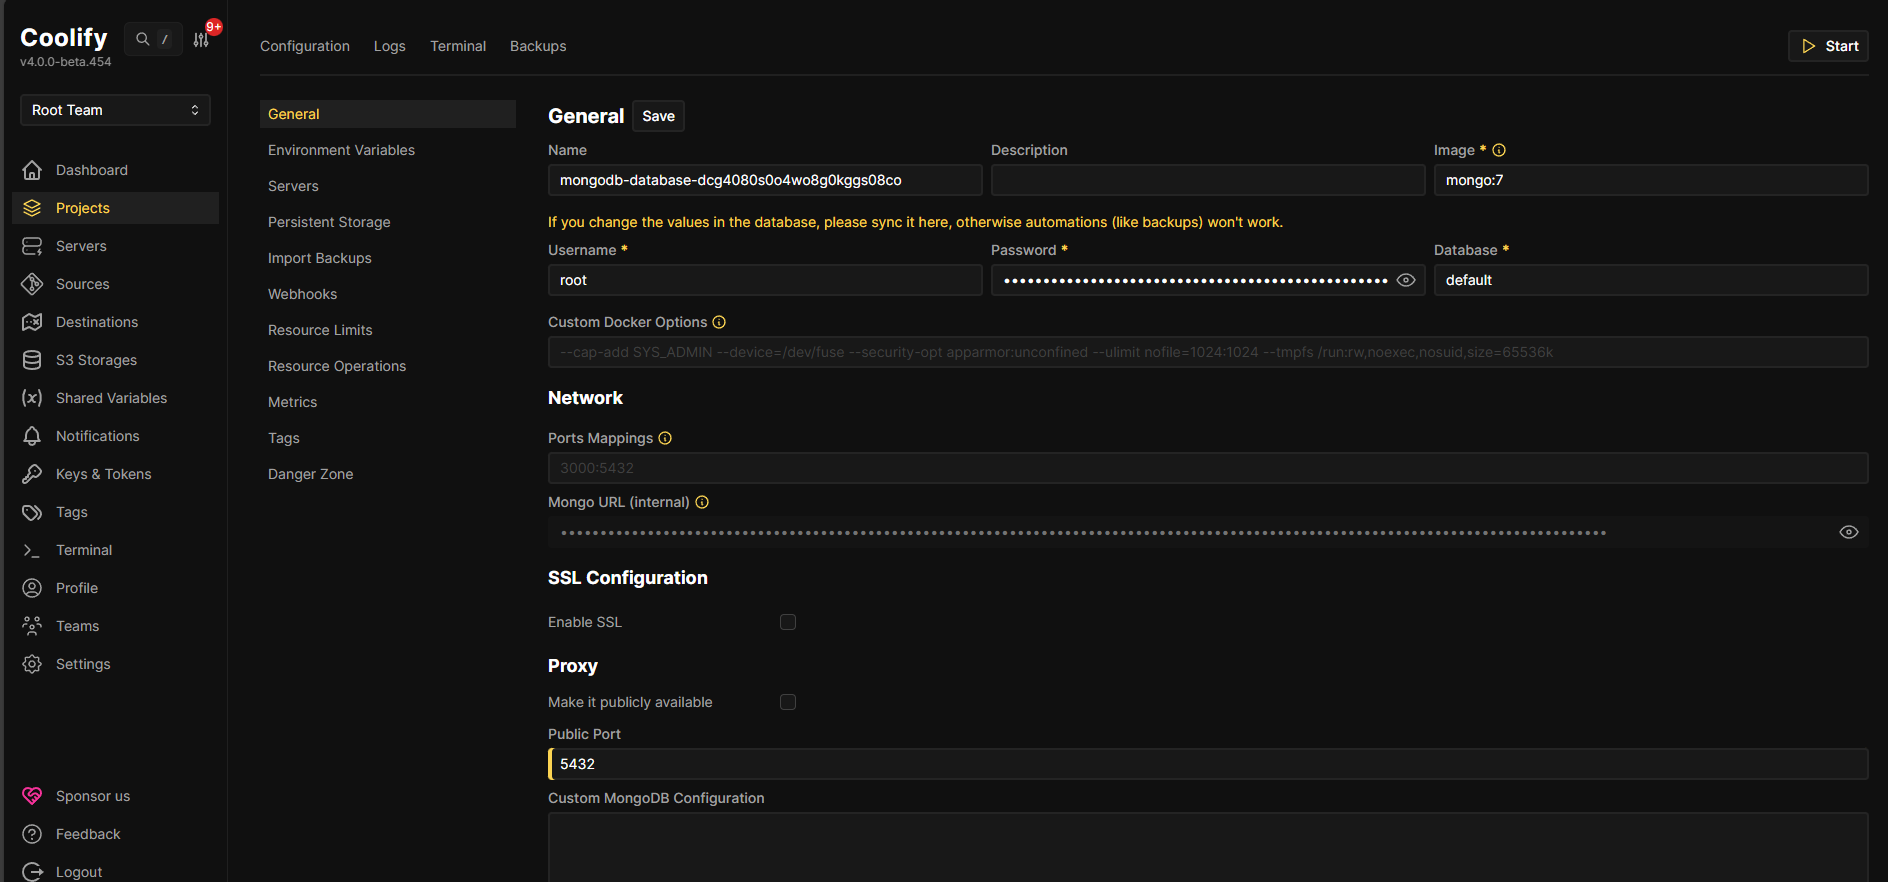
\includegraphics[width=1\textwidth]{24.png}
    \caption{Configurar puertos}
\end{figure}
\FloatBarrier

Ponerle la contraseña generada en la variable de entorno:
\begin{figure}[h!]
    \centering
    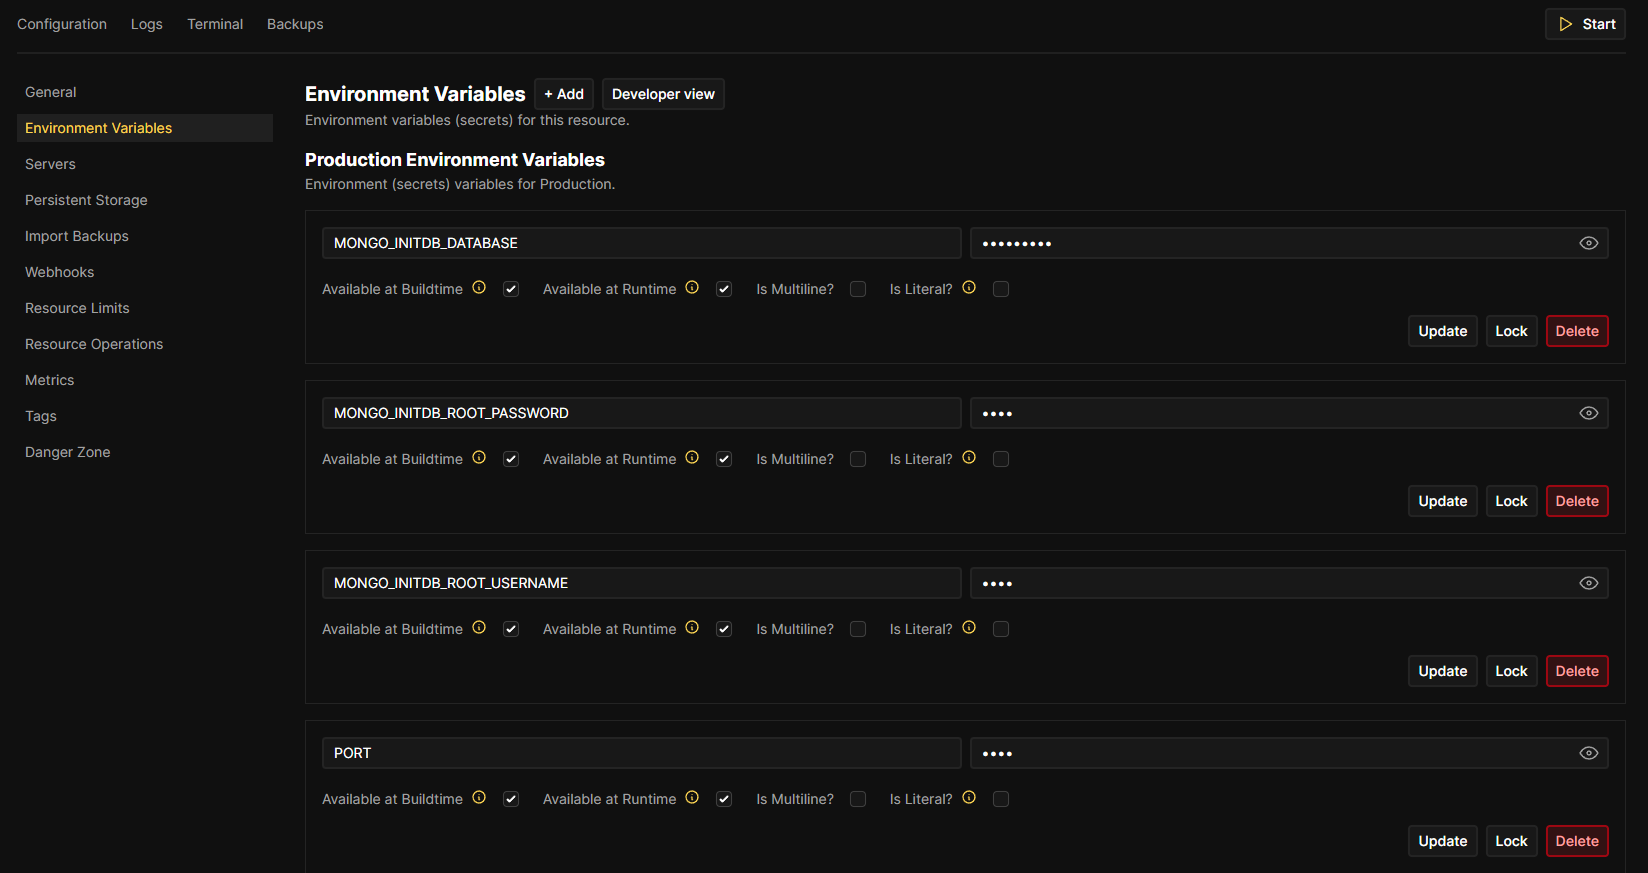
\includegraphics[width=1\textwidth]{25.png}
    \caption{Meter variables de entorno}
\end{figure}
\FloatBarrier

\begin{figure}[h!]
    \centering
    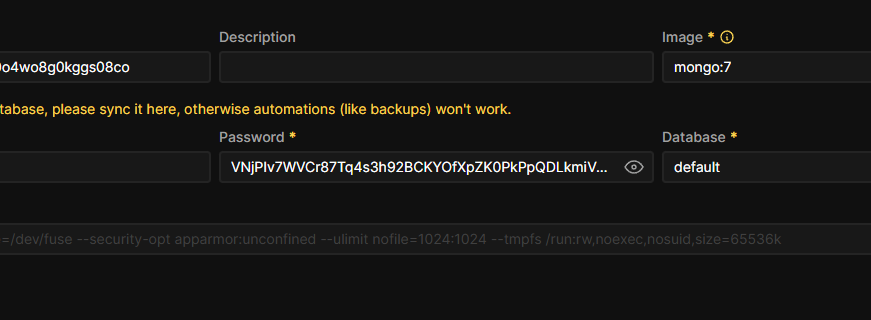
\includegraphics[width=1\textwidth]{26.png}
    \caption{Esta}
\end{figure}
\FloatBarrier

\begin{figure}[h!]
    \centering
    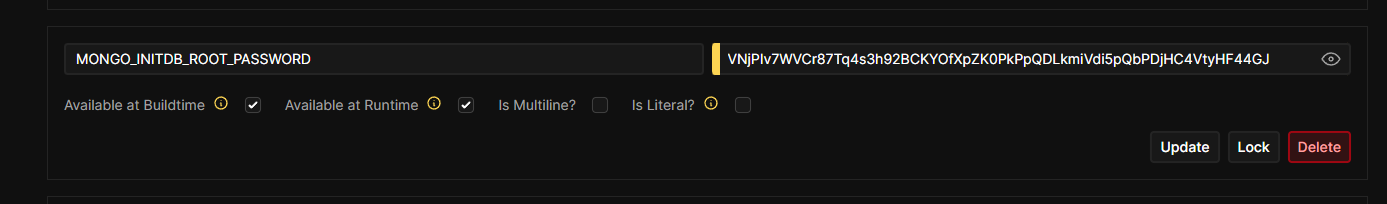
\includegraphics[width=1\textwidth]{27.png}
    \caption{Aquí}
\end{figure}
\FloatBarrier

\begin{figure}[h!]
    \centering
    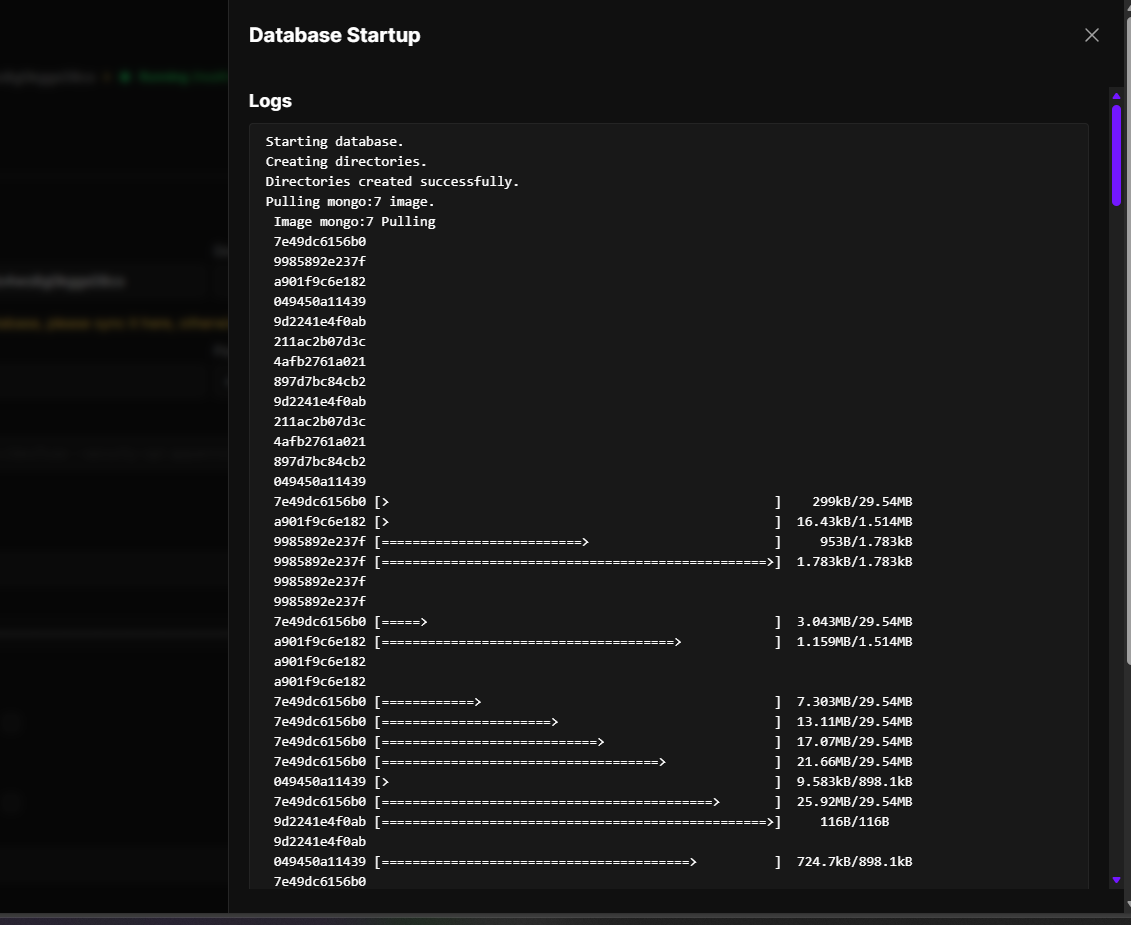
\includegraphics[width=1\textwidth]{28.png}
    \caption{Desplegamos}
\end{figure}
\FloatBarrier

\begin{figure}[h!]
    \centering
    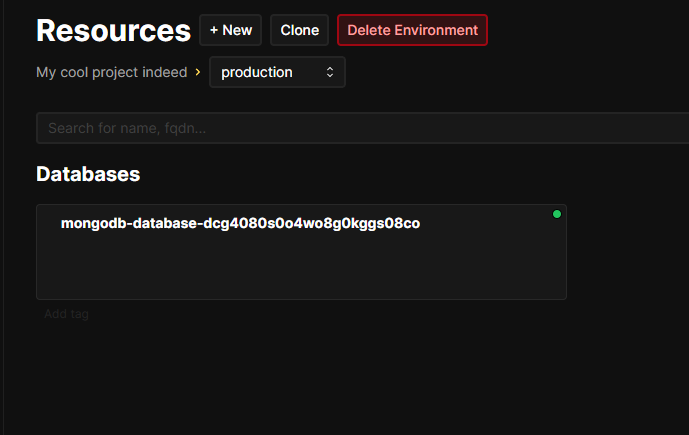
\includegraphics[width=1\textwidth]{29.png}
    \caption{Despliegue correcto}
\end{figure}
\FloatBarrier

Ahora creamos nuevo recurso, en este caso con la API creada en la práctica anterior (\url{https://github.com/1001inchNails/afond_1-4}).

\begin{figure}[h!]
    \centering
    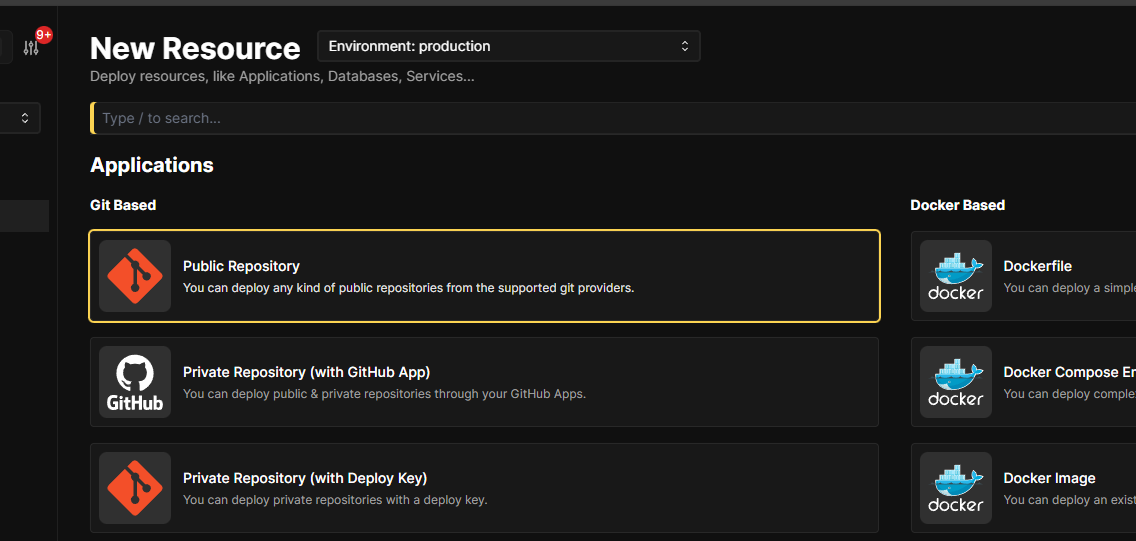
\includegraphics[width=1\textwidth]{30.png}
    \caption{Crear nuevo recurso}
\end{figure}
\FloatBarrier

\begin{figure}[h!]
    \centering
    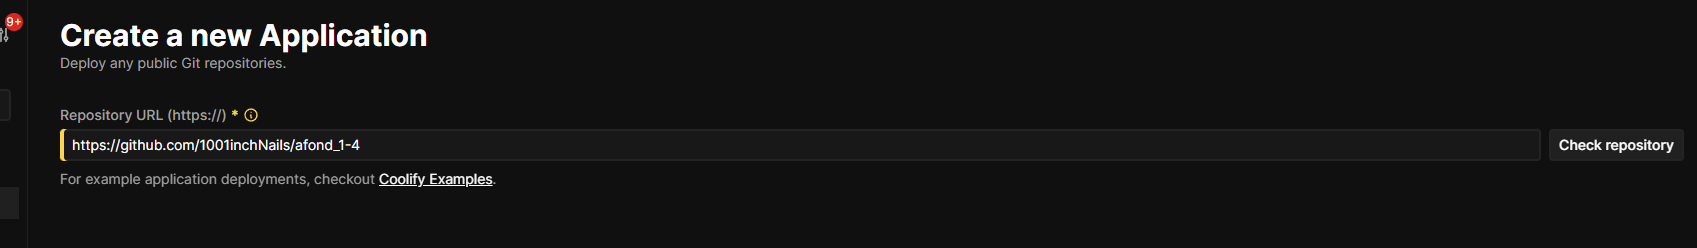
\includegraphics[width=1\textwidth]{31.png}
    \caption{Repositorio público}
\end{figure}
\FloatBarrier

\begin{figure}[h!]
    \centering
    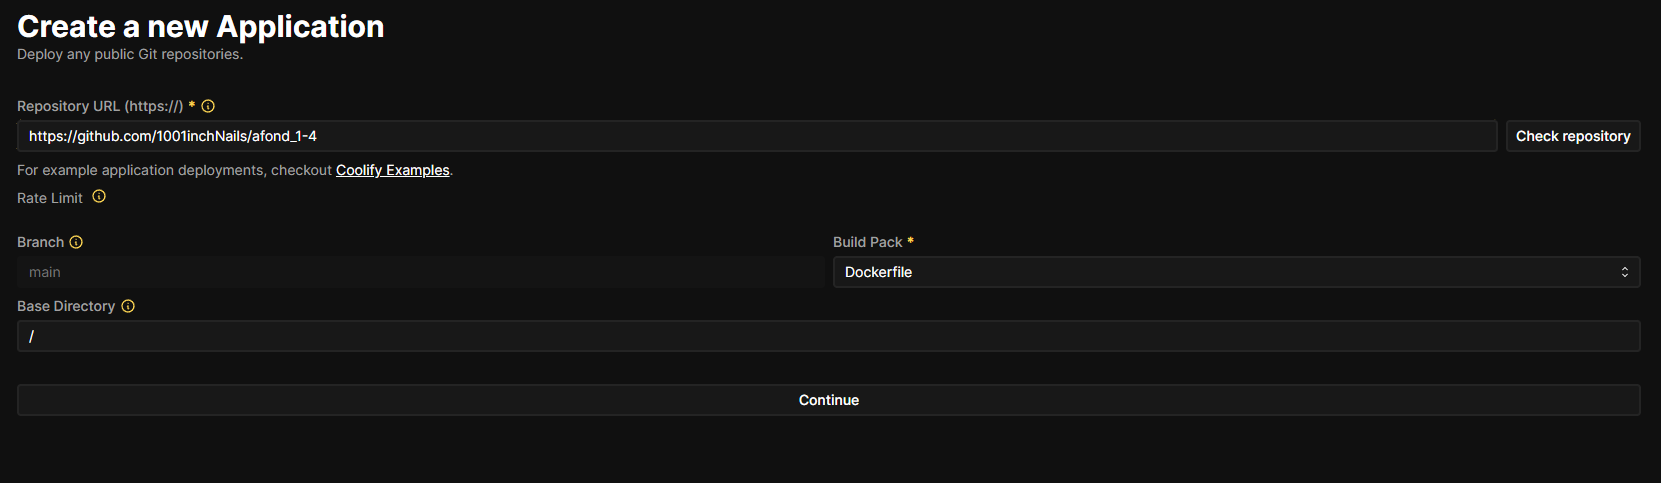
\includegraphics[width=1\textwidth]{32.png}
    \caption{Build: Dockerfile}
\end{figure}
\FloatBarrier

\begin{figure}[h!]
    \centering
    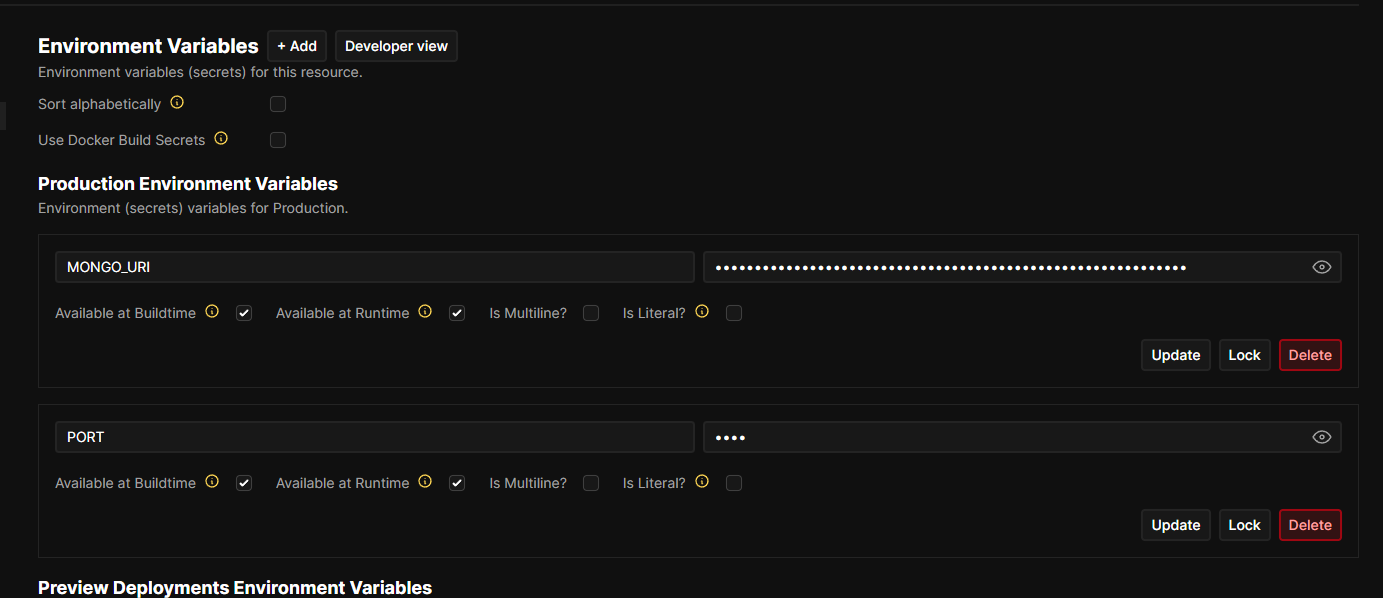
\includegraphics[width=1\textwidth]{33.png}
    \caption{Variables de entorno: meterle el password en MONGO\_URI}
\end{figure}
\FloatBarrier

\begin{figure}[h!]
    \centering
    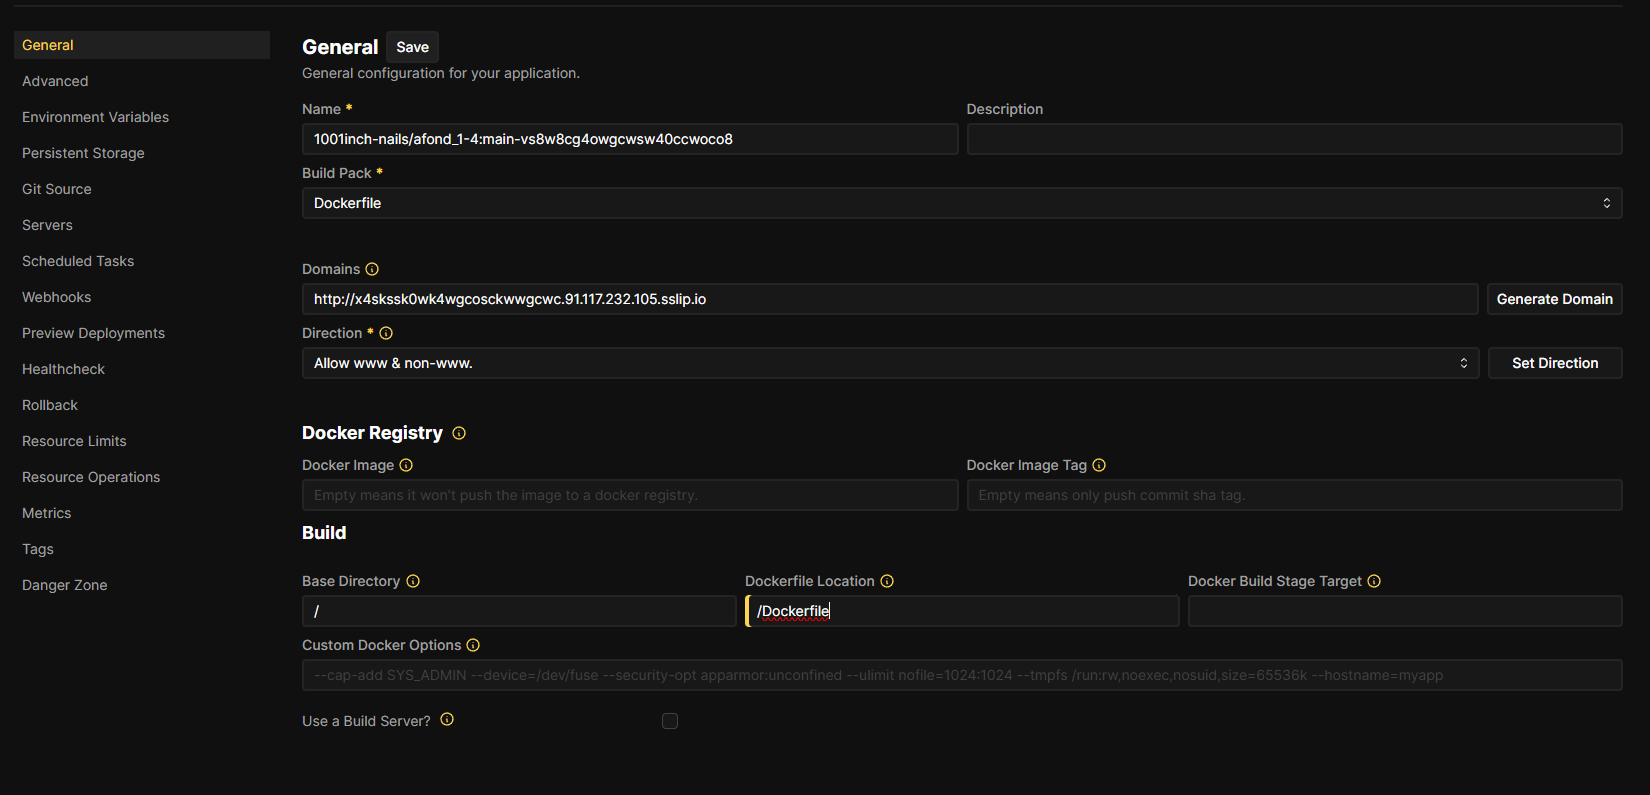
\includegraphics[width=1\textwidth]{34.png}
    \caption{Definir carpeta raiz, y ponerle el mismo puerto que el definido en el código de la API}
\end{figure}
\FloatBarrier

\begin{figure}[h!]
    \centering
    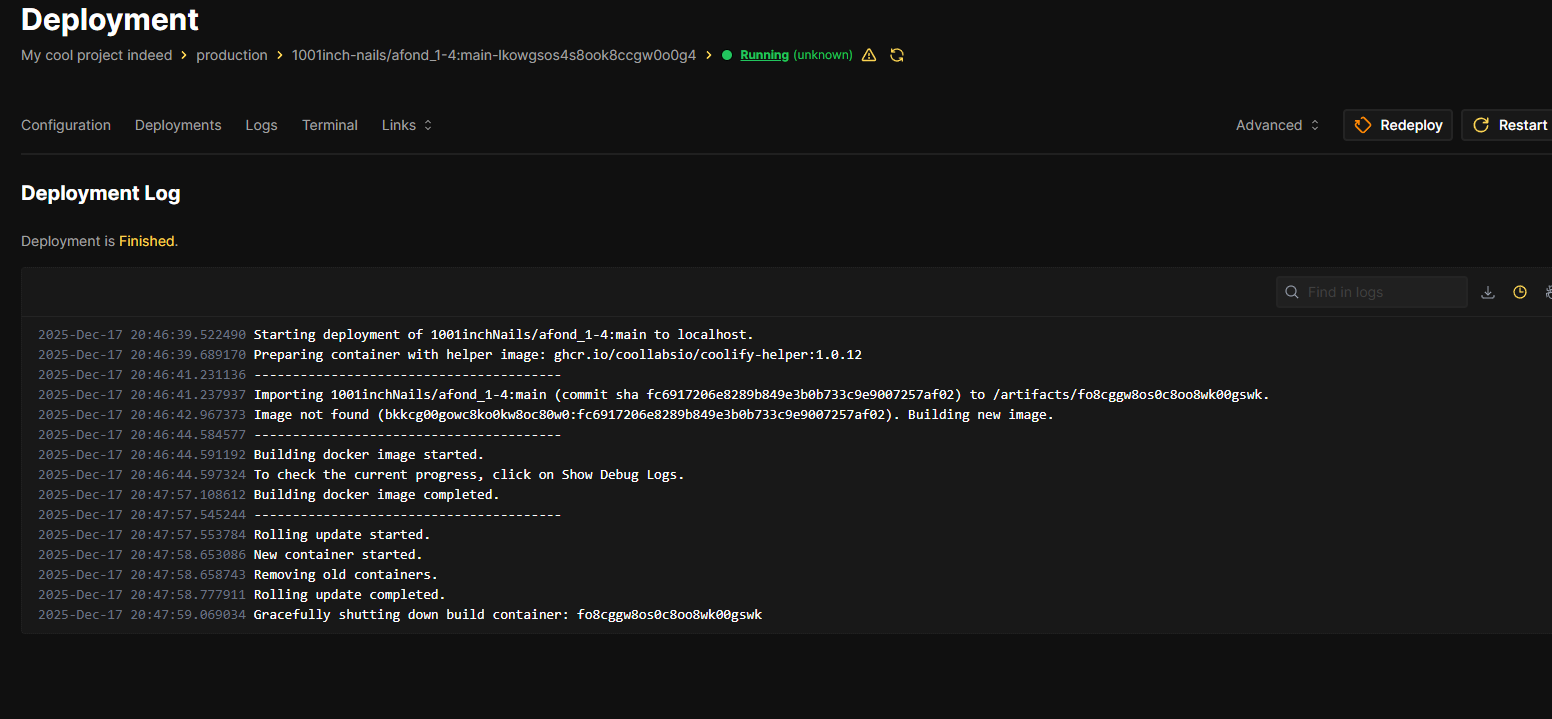
\includegraphics[width=1\textwidth]{35.png}
    \caption{Guardar y desplegar}
\end{figure}
\FloatBarrier

\begin{figure}[h!]
    \centering
    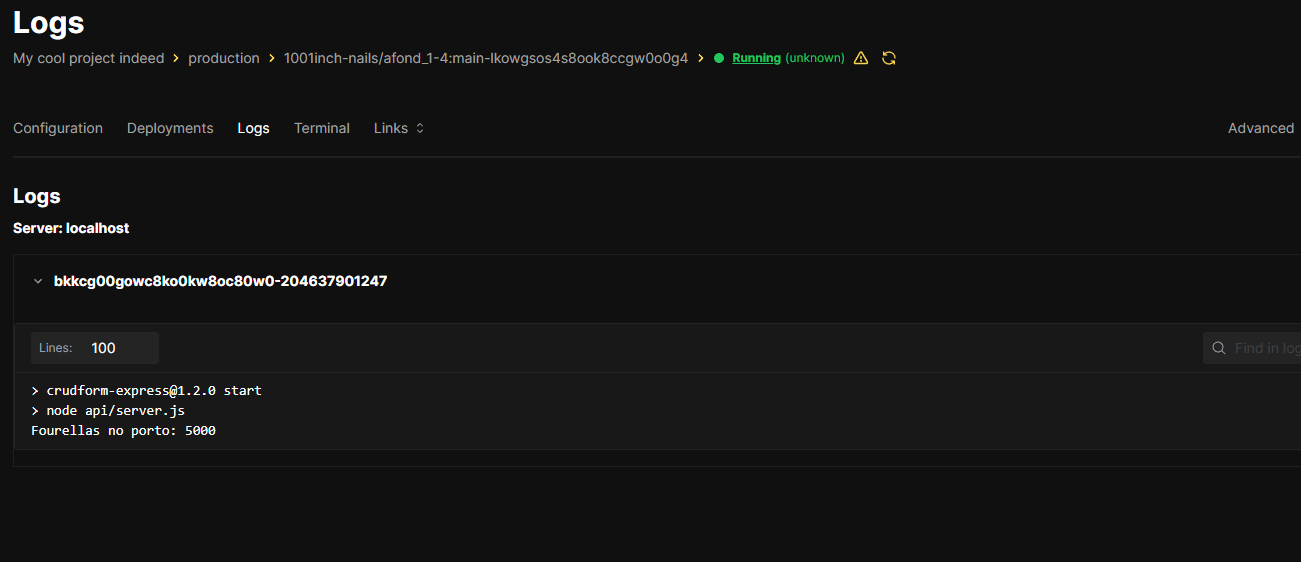
\includegraphics[width=1\textwidth]{36.png}
    \caption{Log}
\end{figure}
\FloatBarrier

Ahora buscamos la IP de la VM:

\begin{figure}[h!]
    \centering
    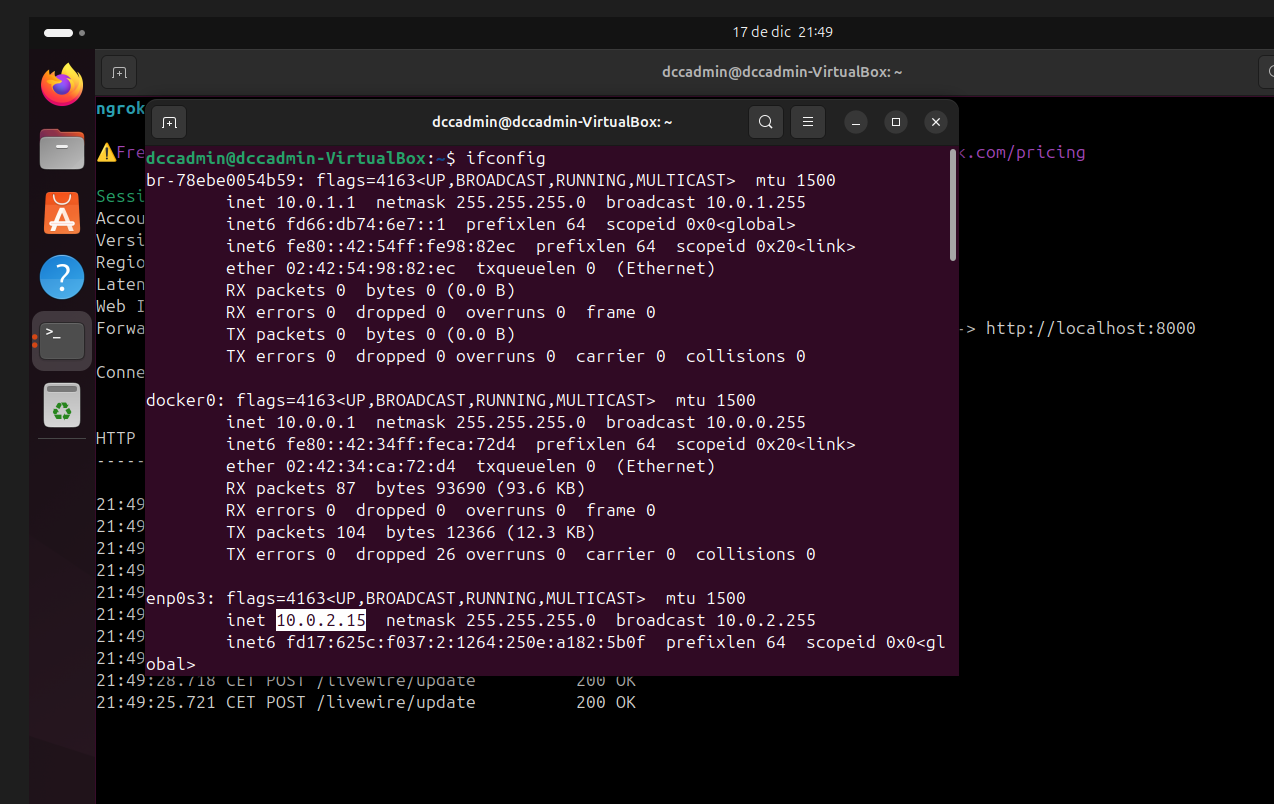
\includegraphics[width=1\textwidth]{37.png}
    \caption{Interfaces de red (enp0s3)}
\end{figure}
\FloatBarrier

Metemos esa IP en el dominio que nos proporciona Coolify:

\begin{figure}[h!]
    \centering
    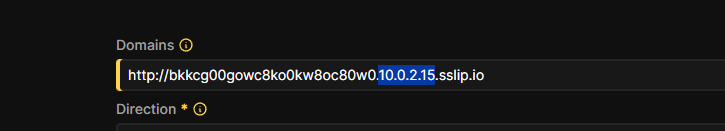
\includegraphics[width=1\textwidth]{38.png}
    \caption{sslip}
\end{figure}
\FloatBarrier

\begin{figure}[h!]
    \centering
    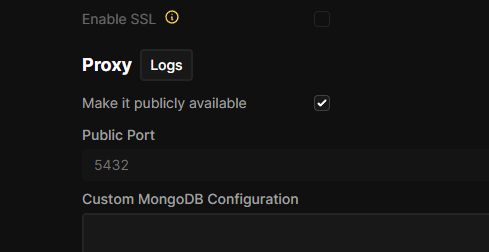
\includegraphics[width=1\textwidth]{39.png}
    \caption{Hacerlo disponible a público}
\end{figure}
\FloatBarrier

\begin{figure}[h!]
    \centering
    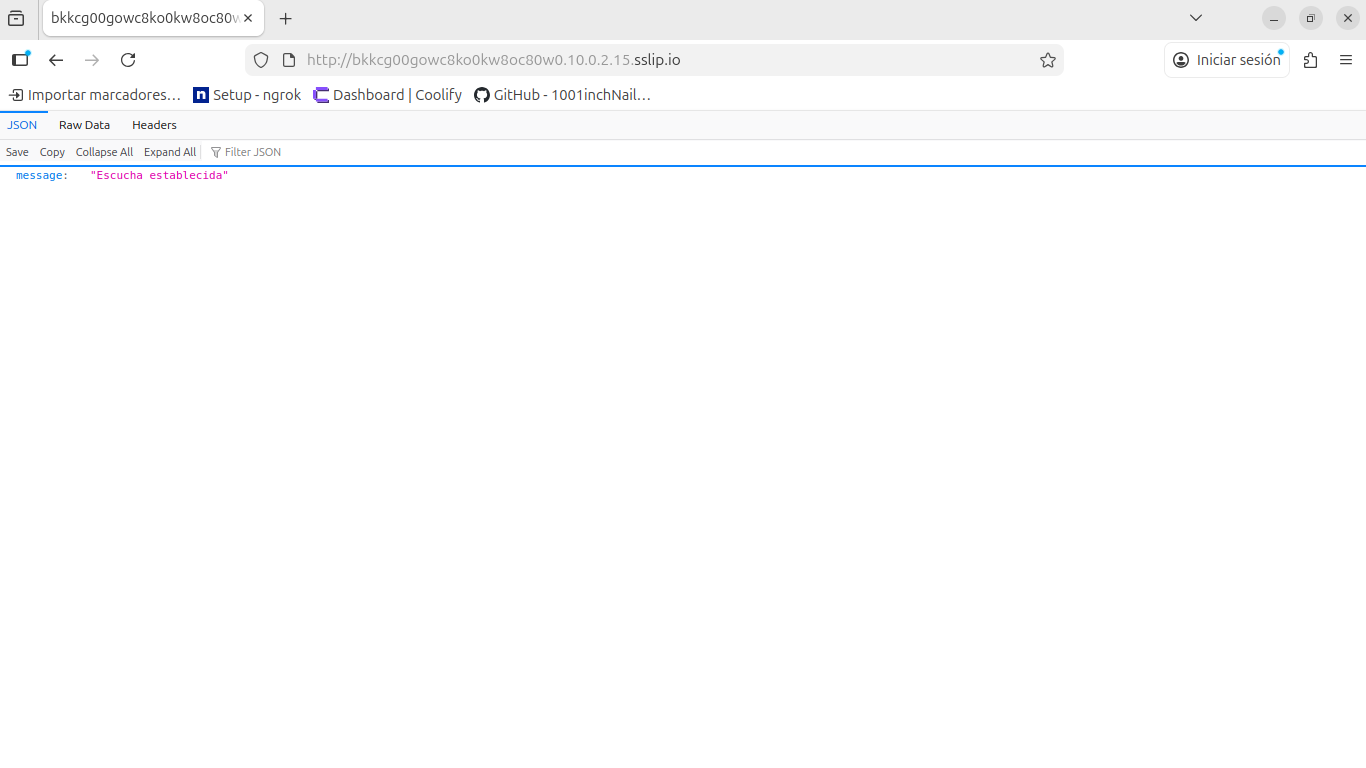
\includegraphics[width=1\textwidth]{41.png}
    \caption{Correcto funcionamiento: VM}
\end{figure}
\FloatBarrier

En este momento se descubrió un problema, en la VM el enlace cargaba correctamente pero no en la máquina host. Esto se debía a que la configuración de red de la VM no estaba en modo puente.

Después de cambiarlo, se procedió a volver a ejecutar \verb|ifconfig| para buscar la IP nueva, meterla en el dominio y, esta vez, cargaba correctamente en host:

\begin{figure}[h!]
    \centering
    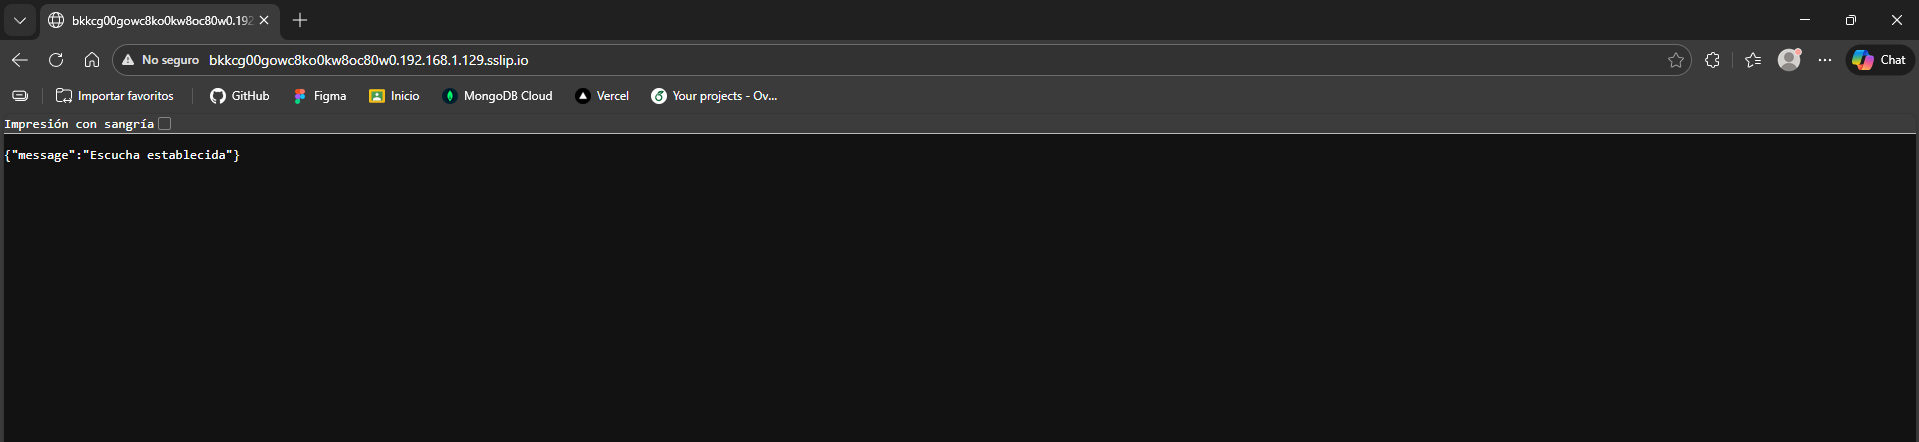
\includegraphics[width=1\textwidth]{42.png}
    \caption{MISSION ACCOMPLISHED}
\end{figure}
\FloatBarrier

\clearpage

\section{Info}
\hyperlink{anchor-indice}{\textbf{Volver}}\\

\textbf{Repositorio}

% \url{https://} (branch \verb|practica4|)\\

\textbf{Comandos:}
\begin{itemize}
    \item Instalar Coolify: \verb|curl -fsSL https://cdn.coollabs.io/coolify/install.sh | sudo bash|
    \item Instalar Ngrok: \begin{verbatim}
      curl -sSL https://ngrok-agent.s3.amazonaws.com/ngrok.asc
      sudo tee /etc/apt/trusted.gpg.d/ngrok.asc >/dev/null
      && echo "deb https://ngrok-agent.s3.amazonaws.com bookworm main"
      | sudo tee /etc/apt/sources.list.d/ngrok.list
      && sudo apt update
      && sudo apt install ngrok
      \end{verbatim}
    \item Añadir authtoken: \verb|ngrok config add-authtoken <authtoken>|
    \item Información contenedores Docker: \verb|docker ps|
    \item IP de contenedor: \verb|docker inspect -f '{{range .NetworkSettings.Networks}}{{.IPAddress}}{{end}}' idDelContainer|
    \item Exponer API test con Ngrok: \verb|ngrok http <ip>:<puerto>|
    \item Exponer puerto con Ngrok: \verb|ngrok http <puerto>|
    \item Interfaces de red: \verb|ifconfig|
    
\end{itemize}

\end{document}
